\documentclass[../AnalisiDeiRequisiti.tex]{subfiles}
\begin{document}
	\section{Casi d'uso}
	I seguenti casi d'uso sono frutto dell'analisi del capitolato, della discussione degli
	\analisti\ e degli incontri con	\proponente\ ed il committente \vardanega.
	Tali casi d'uso hanno quindi origine sia interna che esterna al gruppo.\\
	Le aspettative di esperienza utente derivano dalla sua conoscenza del
	linguaggio UML.\\
	Ciascun caso d'uso è classificato gerarchicamente con la seguente dicitura:
	\begin{center}
		UC[Codice del padre].[Codice identificativo]
	\end{center}
	Il codice identificativo può includere diversi livelli di gerarchia che saranno
	separati da un punto.
	\subsection{Attori}
		L'unico attore che interagisce con il nostro sistema è l'utente.
		\begin{figure} [H]
			\centering
			
\includegraphics[scale=0.45]{./Figures/utente.png}
			\caption{Diagramma attori}\label{}
		\end{figure}
	\subsection{Funzionalità principali dell'editor UML}
		\begin{figure} [H]
			\centering
			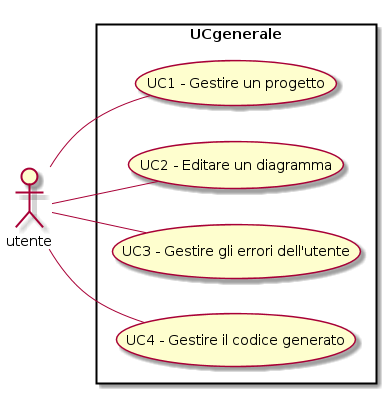
\includegraphics[scale=0.45]{./Figures/UCgenerale.png}
			\caption{Diagramma UC principali}\label{}
		\end{figure}
	\subsection{Caso d'uso UC1: Gestire un progetto}
		\begin{figure} [H]
			\centering
			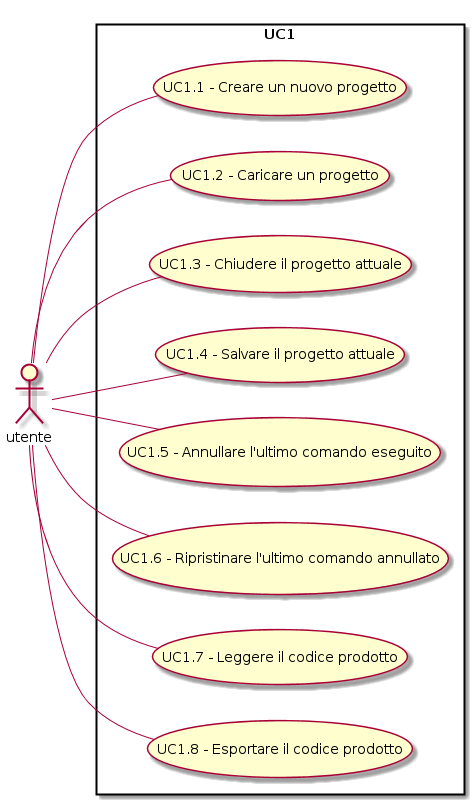
\includegraphics[scale=0.45]{./Figures/UC1.png}
			\caption{Diagramma UC1}\label{}
		\end{figure}
	\begin{itemize}
		\item \textbf{Attori}: Utente
		\item \textbf{Descrizione}: L'utente vuole gestire il progetto su cui lavorare;
		\item \textbf{Precondizione}: Il programma si è avviato correttamente ed è pronto a ricevere un input dall'utente;
		\item \textbf{Flusso principale degli eventi}: \begin{itemize}
			\item L'utente può creare un nuovo progetto (UC1.1);
			\item L'utente può caricare un progetto (UC1.2);
			\item L'utente può chiudere il progetto attuale (UC1.3);
			\item L'utente può salvare il progetto attuale (UC1.4).
			%\item L'utente può annullare l'ultimo comando eseguito (UC:);
			%\item L'utente può ripristinare l'ultimo comando annullato (UC:);
			%\item L'utente può leggere il codice prodotto (UC:);
			%\item L'utente può esportare il codice prodotto (UC:);
		\end{itemize}
		\item \textbf{Postcondizione}: È stata completata l'operazione sul progetto desiderata.
	\end{itemize}
	\subsection{Caso d'uso UC1.1: Creare un nuovo progetto}
	\begin{itemize}
		\item \textbf{Attori}: Utente
		\item \textbf{Descrizione}: L'utente vuole creare un nuovo progetto;
		\item \textbf{Precondizione}: Il programma si è avviato correttamente ed è pronto a ricevere un input dall'utente;
		\item \textbf{Flusso principale degli eventi}: L'utente crea un nuovo progetto. Ne inserisce il nome e il sistema crea automaticamente un diagramma dei package vuoto che viene mostrato sullo schermo;
		\item \textbf{Postcondizione}: È stato creato un nuovo progetto che è pronto ad essere modificato.
	\end{itemize}
	\subsection{Caso d'uso UC1.2: Caricare un progetto}
	\begin{itemize}
		\item \textbf{Attori}: Utente
		\item \textbf{Descrizione}: L'utente vuole caricare un progetto precedentemente creato;
		\item \textbf{Precondizione}: Il programma si è avviato correttamente ed è pronto a ricevere un input dall'utente;
		\item \textbf{Flusso principale degli eventi}: L'utente carica un progetto precedentemente creato;
		\item \textbf{Postcondizione}: È stato caricato un nuovo progetto che è pronto ad essere modificato.
	\end{itemize}
	\subsection{Caso d'uso UC1.3: Chiudere il progetto attuale}
	\begin{itemize}
		\item \textbf{Attori}: Utente
		\item \textbf{Descrizione}: L'utente vuole chiudere il progetto correntemente aperto;
		\item \textbf{Precondizione}: Il programma è in attesa di un comando dall'utente e ha un progetto aperto;
		\item \textbf{Flusso principale degli eventi}: L'utente chiude il progetto correntemente aperto;
		\item \textbf{Postcondizione}: Il progetto aperto in precedenza è stato chiuso.
	\end{itemize}
	\subsection{Caso d'uso UC1.4: Salvare il progetto attuale}
	\begin{itemize}
		\item \textbf{Attori}: Utente
		\item \textbf{Descrizione}: L'utente vuole salvare il lavoro fatto fino a quel momento;
		\item \textbf{Precondizione}: Nelle schermate degli editor messi a disposizione del programma sono stati disegnati i diagrammi che rappresentano il codice desiderato;
		\item \textbf{Flusso principale degli eventi}: L'utente salva il lavoro fatto fino a quel momento;
		\item \textbf{Postcondizione}: In una cartella a scelta dell'utente il programma ha generato un file di tipo proprietario contenente tutte le informazioni necessarie per ripristinarne lo stato attuale.
	\end{itemize}
	\subsection{Caso d'uso UC2: Editare un diagramma}
		\begin{figure} [H]
			\centering
			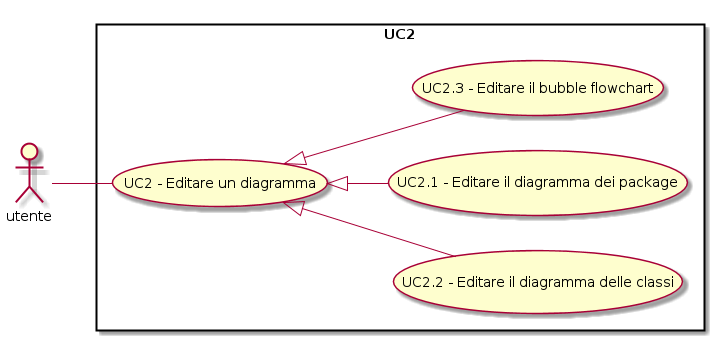
\includegraphics[scale=0.45]{./Figures/UC2.png}
			\caption{Diagramma UC2}\label{}
		\end{figure}
	\begin{itemize}
		\item \textbf{Attori}: Utente
		\item \textbf{Descrizione}: L'utente vuole editare un diagramma;
		\item \textbf{Precondizione}: L'utente ha avviato correttamente il programma ed ha aperto un progetto. Il sistema è pronto per accettare le modifiche dell'utente;
		\item \textbf{Flusso principale degli eventi}: \begin{itemize}
			\item L'utente può editare il diagramma dei package (UC2.1);
			\item L'utente può editare il diagramma delle classi (UC2.2);
			\item L'utente può editare il diagramma delle attività (UC2.3);
		\end{itemize}
		\item \textbf{Postcondizione}: Il sistema apporta le modifiche desiderate al diagramma scelto.
	\end{itemize}
	\subsection{Caso d'uso UC2.1: Editare il diagramma dei package}
	\begin{figure} [H]
		\centering
		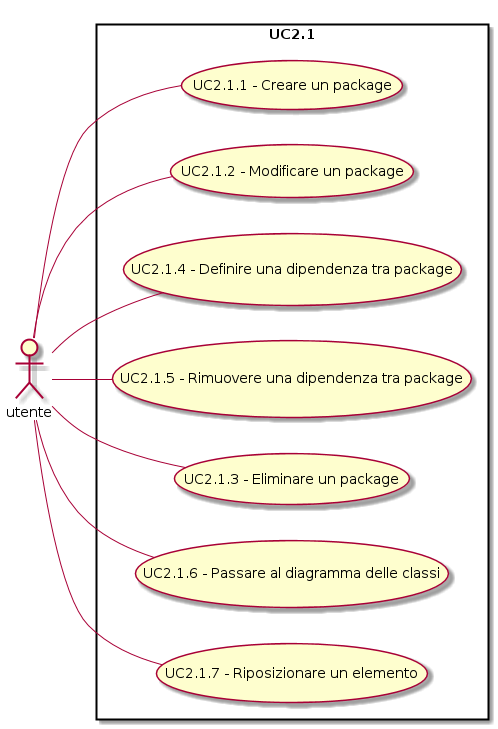
\includegraphics[scale=0.45]{./Figures/UC2-1.png}
		\caption{Diagramma UC2.1}\label{}
	\end{figure}
	\begin{itemize}
		\item \textbf{Attori}: Utente
		\item \textbf{Descrizione}: L'utente vuole editare il diagramma dei package;
		\item \textbf{Precondizione}: Nella schermata dell'editor del diagramma dei package il sistema è pronto a ricevere un comando dall'utente;
		\item \textbf{Flusso principale degli eventi}: \begin{itemize}
			\item L'utente può creare un package (UC2.1.1);
			\item L'utente può modificare un package (UC2.1.2);
			\item L'utente può rimuovere un package (UC2.1.3);
			\item L'utente può definire una dipendenza tra package (UC2.1.4);
			\item L'utente può rimuovere una dipendenza tra package (UC2.1.5);
			\item L'utente può passare dal diagramma dei package al diagramma delle classi (UC2.1.6);
			\item L'utente può riposizionare un elemento (UC2.1.7).
		\end{itemize}
		\item \textbf{Scenari alternativi}: Viene annullata la modifica, il diagramma rimane nello stato precedente al tentativo di modifica;
		\item \textbf{Postcondizione}: L'utente ha editato diagramma dei package come voluto e il sistema è pronto a ricevere un nuovo comando.
	\end{itemize}
	\subsection{Caso d'uso UC2.1.1: Creare un package}
	\begin{itemize}
		\item \textbf{Attori}: Utente
		\item \textbf{Descrizione}: L'utente vuole creare un package;
		\item \textbf{Precondizione}: Nella schermata dell'editor del diagramma dei package il sistema è pronto a ricevere un comando dall'utente;
		\item \textbf{Flusso principale degli eventi}: L'utente crea un package;
		\item \textbf{Postcondizione}: Nella schermata dell'editor del diagramma dei package è visualizzato il diagramma a cui è stato aggiunto un nuovo package.
	\end{itemize}
	\subsection{Caso d'uso UC2.1.2: Modificare un package}
	\begin{figure} [H]
		\centering
		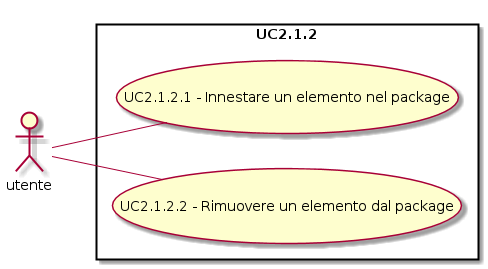
\includegraphics[scale=0.45]{./Figures/UC2-1-2.png}
		\caption{Diagramma UC2.1.2}\label{}
	\end{figure}
	\begin{itemize}
		\item \textbf{Attori}: Utente
		\item \textbf{Descrizione}: L'utente vuole modificare un package;
		\item \textbf{Precondizione}: Nell'editor del diagramma dei package è stato selezionato un package che l'utente desidera modificare;
		\item \textbf{Flusso principale degli eventi}: \begin{itemize}
			\item L'utente modifica il package;
			\item L'utente può innestare un elemento nel package (UC2.1.2.1);
			\item L'utente può rimuovere un elemento dal package (UC2.1.2.2);
		\end{itemize}
		\item \textbf{Scenari alternativi}: Viene annullata la modifica, il sistema	rimane nello stato precedente al tentativo di modifica;
		\item \textbf{Postcondizione}: Nell'editor del diagramma dei package è visualizzato il diagramma dove sono state apportate le modifiche al package e il sistema è pronto a ricevere un nuovo comando.
	\end{itemize}
	\subsection{Caso d'uso UC2.1.2.1: Innestare un elemento nel package}
	\begin{itemize}
		\item \textbf{Attori}: Utente
		\item \textbf{Descrizione}: L'utente vuole innestare un elemento all'interno di un package;
		\item \textbf{Precondizione}: Nell'editor del diagramma dei package il sistema è pronto ad effettuare l'innesto;
		\item \textbf{Flusso principale degli eventi}: L'utente innesta un elemento all'interno del package;
		\item \textbf{Postcondizione}: Nell'editor del diagramma dei package è visualizzato il diagramma dove è stato effettuato l'innesto e il sistema è pronto a ricevere un nuovo comando.
	\end{itemize}
	\subsection{Caso d'uso UC2.1.2.2: Rimuovere un elemento dal package}
	\begin{itemize}
		\item \textbf{Attori}: Utente
		\item \textbf{Descrizione}: L'utente vuole rimuovere un elemento da un package;
		\item \textbf{Precondizione}: Nell'editor del diagramma dei package è selezionato l'elemento che l'utente desidera rimuovere;
		\item \textbf{Flusso principale degli eventi}: L'utente rimuove un elemento da un package;
		\item \textbf{Postcondizione}: Nell'editor del diagramma dei package è visualizzato il diagramma dove è stato rimosso l'elemento e il sistema è pronto a ricevere un nuovo comando.
	\end{itemize}
	\subsection{Caso d'uso UC2.1.3: Eliminare un package}
	\begin{itemize}
		\item \textbf{Attori}: Utente
		\item \textbf{Descrizione}: L'utente vuole eliminare un package;
		\item \textbf{Precondizione}: Nell'editor del diagramma dei package è selezionato il package che l'utente desidera rimuovere;
		\item \textbf{Flusso principale degli eventi}: L'utente elimina un package;
		\item \textbf{Postcondizione}: Nell'editor del diagramma dei package è visualizzato il diagramma dove è stato eliminato il package e il sistema è pronto a ricevere un nuovo comando.
	\end{itemize}
	\subsection{Caso d'uso UC2.1.4: Definire una dipendenza tra package}
	\begin{itemize}
		\item \textbf{Attori}: Utente
		\item \textbf{Descrizione}: L'utente vuole definire una dipendenza tra due package;
		\item \textbf{Precondizione}: Nell'editor del diagramma dei package il sistema è pronto a creare la dipendenza che l'utente desidera definire;
		\item \textbf{Flusso principale degli eventi}: L'utente definisce una dipendenza tra due package;
		\item \textbf{Postcondizione}: Nell'editor del diagramma dei package del sistema è visualizzato il diagramma dove è stata definita la dipendenza e il sistema è pronto a ricevere un nuovo comando.
	\end{itemize}
	\subsection{Caso d'uso UC2.1.5: Rimuovere una dipendenza tra package}
	\begin{itemize}
		\item \textbf{Attori}: Utente
		\item \textbf{Descrizione}: L'utente vuole rimuovere una dipendenza tra due package;
		\item \textbf{Precondizione}: Nell'editor del diagramma dei package il sistema è pronto a eliminare la dipendenza che l'utente desidera rimuovere;
		\item \textbf{Flusso principale degli eventi}: L'utente rimuove una dipendenza tra due package;
		\item \textbf{Postcondizione}: Nell'editor del diagramma dei package è visualizzato il diagramma dove è stata rimossa la dipendenza e il sistema è pronto a ricevere un nuovo comando.
	\end{itemize}
	\subsection{Caso d'uso UC2.1.6: Passare dal diagramma dei package al diagramma delle classi}
	\begin{itemize}
		\item \textbf{Attori}: Utente
		\item \textbf{Descrizione}: L'utente vuole tornare alla schermata dell'editor del diagramma delle classi di un particolare package;
		\item \textbf{Precondizione}: Il sistema visualizza l'editor del diagramma dei package;
		\item \textbf{Flusso principale degli eventi}: L'utente torna alla schermata dell'editor del diagramma delle classi di un particolare package;
		\item \textbf{Postcondizione}: Il sistema visualizza nell'editor del diagramma delle classi il package desiderato.
	\end{itemize}
	\subsection{Caso d'uso UC2.1.7: Riposizionare un elemento}
	\begin{itemize}
		\item \textbf{Attori}: Utente
		\item \textbf{Descrizione}: L'utente vuole cambiare la posizione di un elemento all'interno del diagramma;
		\item \textbf{Precondizione}: L'utente si trova nella schermata dell'editor del diagramma dei package e il sistema è pronto a ricevere un comando dall'utente;
		\item \textbf{Flusso principale degli eventi}: L'utente riposiziona l'elemento;
		\item \textbf{Postcondizione}: Il sistema visualizza il diagramma con l'elemento riposizionato correttamente;
	\end{itemize}
	\subsection{Caso d'uso UC2.2: Editare il diagramma delle classi}
	\begin{figure} [H]
		\centering
		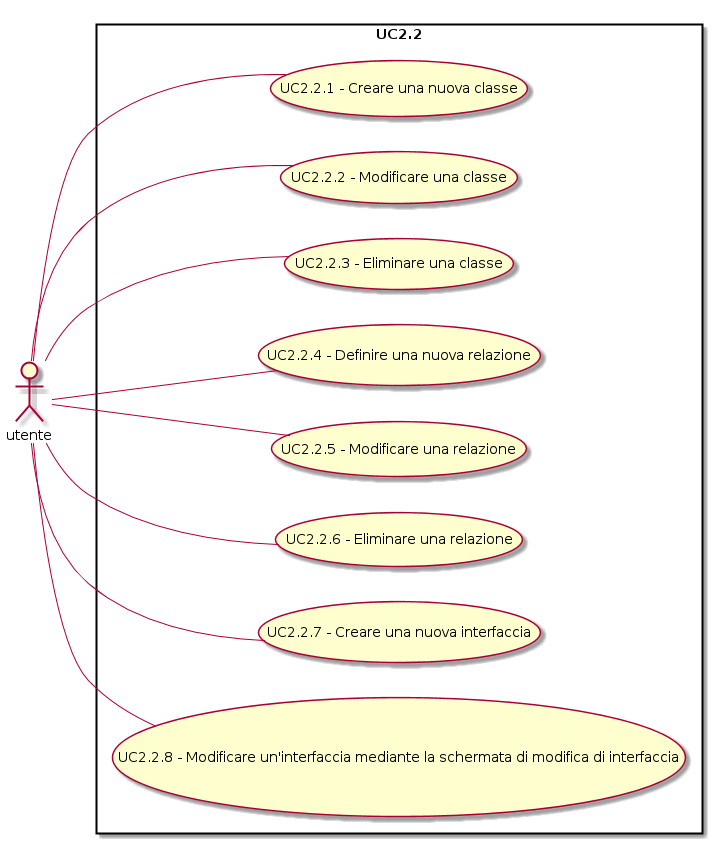
\includegraphics[scale=0.45]{./Figures/UC2-2parte1.png}
		\caption{Diagramma UC2.2 prima parte}\label{}
	\end{figure}
	\begin{figure} [H]
		\centering
		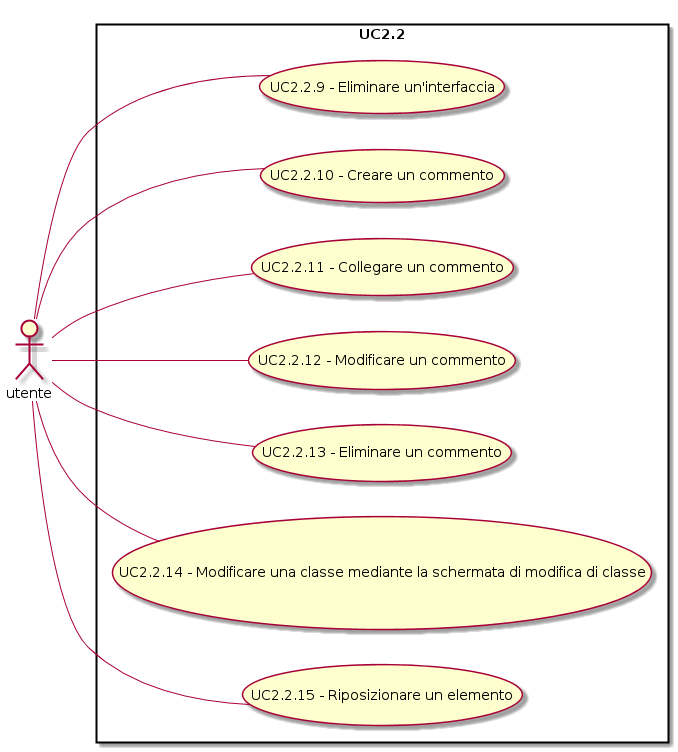
\includegraphics[scale=0.45]{./Figures/UC2-2parte2.png}
		\caption{Diagramma UC2.2 seconda parte}\label{}
	\end{figure}
	\begin{itemize}
		\item \textbf{Attori}: Utente
		\item \textbf{Descrizione}: L'utente vuole editare il diagramma delle classi;
		\item \textbf{Precondizione}: Nella schermata dell'editor del diagramma delle classi il sistema è pronto a ricevere un comando dall'utente;
		\item \textbf{Flusso principale degli eventi}: \begin{itemize}
			\item L'utente può creare una nuova classe (UC2.2.1);
			\item L'utente può modificare una classe (UC2.2.2);
			\item L'utente può eliminare una classe (UC2.2.3);
			\item L'utente può definire una nuova relazione (UC2.2.4);
			\item L'utente può modificare una relazione (UC2.2.5);
			\item L'utente può eliminare una relazione (UC2.2.6);
			\item L'utente può creare una nuova interfaccia (UC2.2.7);
			\item L'utente può modificare un'interfaccia mediante la schermata di modifica dell'interfaccia (UC2.2.8);
			\item L'utente può eliminare un'interfaccia (UC2.2.9);
			\item L'utente può creare un commento (UC2.2.10);
			\item L'utente può collegare un commento (UC2.2.11);
			\item L'utente può modificare un commento (UC2.2.12);
			\item L'utente può eliminare un commento (UC2.2.13);
			\item L'utente può modificare una classe mediante la schermata di modifica di una classe (UC2.2.14);
			\item L'utente può riposizionare un elemento (UC2.2.15);
		\end{itemize}
		\item \textbf{Scenari alternativi}: Viene annullata la modifica, il sistema rimane nello stato precedente al tentativo di modifica;
		\item \textbf{Postcondizione}: Il sistema apporta le modifiche desiderate al diagramma delle classi.
	\end{itemize}
	\subsection{Caso d'uso UC2.2.1: Creare una nuova classe}
	\begin{itemize}
		\item \textbf{Attori}: Utente
		\item \textbf{Descrizione}: L'utente può aggiungere una nuova classe vuota al diagramma delle classi;
		\item \textbf{Precondizione}: Il programma è in esecuzione con un progetto aperto nel diagramma delle classi;
		\item \textbf{Flusso principale degli eventi}: L'utente aggiunge una nuova classe vuota al diagramma delle classi;
		\item \textbf{Postcondizione}: Viene aggiunta una nuova classe al diagramma delle classi.
	\end{itemize}
	\subsection{Caso d'uso UC2.2.2: Modificare una classe}
	\begin{itemize}
		\item \textbf{Attori}: Utente
		\item \textbf{Descrizione}: L'utente vuole apportare modifiche minori ad una classe;
		\item \textbf{Precondizione}: L'utente ha avviato il programma, sta visualizzando il diagramma delle classi e ha selezionato la classe che vuole modificare;
		\item \textbf{Flusso principale degli eventi}: \begin{itemize}
			\item L'utente apporta le modifiche minori desiderate;
			\item L'utente può aprire la schermata di modifica di classe corrispondente;
		\end{itemize}
		\item \textbf{Postcondizione}: Le modifiche vengono applicate alla classe nel diagramma delle classi.
	\end{itemize}
	\subsection{Caso d'uso UC2.2.3: Eliminare una classe}
	\begin{itemize}
		\item \textbf{Attori}: Utente
		\item \textbf{Descrizione}: L'utente vuole eliminare una classe;
		\item \textbf{Precondizione}: Esiste una classe che l'utente desidera eliminare;
		\item \textbf{Flusso principale degli eventi}: L'utente elimina una classe;
		\item \textbf{Postcondizione}: La classe non è più visualizzata nell'editor del diagramma delle classi.
	\end{itemize}
	\subsection{Caso d'uso UC2.2.4: Definire una nuova relazione}
	\begin{figure} [H]
		\centering
		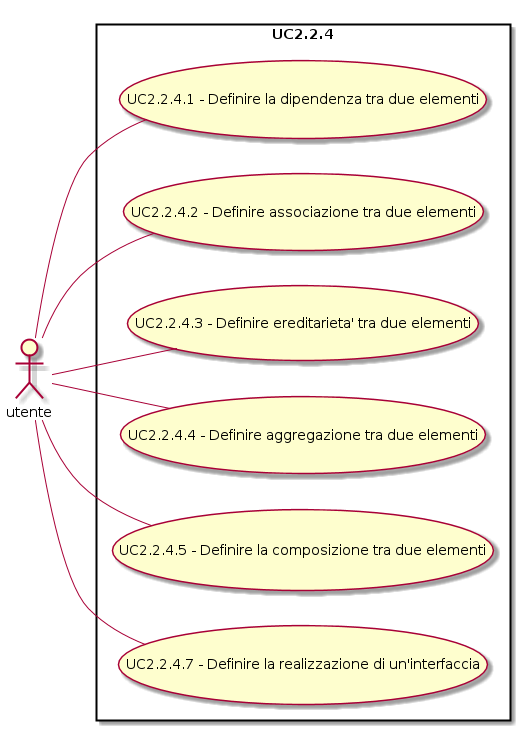
\includegraphics[scale=0.45]{./Figures/UC2-2-4.png}
		\caption{Diagramma UC2.2.4}\label{}
	\end{figure}
	\begin{itemize}
		\item \textbf{Attori}: Utente
		\item \textbf{Descrizione}: L'utente vuole definire una relazione tra due elementi.
		\item \textbf{Precondizione}: Sono presenti due elementi e l'utente desidera che presentino una relazione l'una dall'altra.
		\item \textbf{Flusso principale degli eventi}: \begin{itemize}
			\item L'utente vuole definire la dipendenza tra due elementi (UC2.2.4.1);
			\item L'utente vuole definire l'associazione tra due elementi (UC2.2.4.2);
			\item L'utente vuole definire l'ereditarietà tra due elementi (UC2.2.4.3);
			\item L'utente vuole definire l'aggregazione tra due elementi (UC2.2.4.4);
			\item L'utente vuole definire la composizione tra due elementi (UC2.2.4.5);
			\item L'utente vuole definire il raffinamento di una classe parametrica (UC2.2.4.6);
			\item L'utente vuole definire la realizzazione di un'interfaccia (UC2.2.4.7).
			\end{itemize}
				\item \textbf{Postcondizione}: I due elementi vengono messi in relazione.
			\end{itemize}
			\subsection{Caso d'uso UC2.2.4.1: Definire la dipendenza tra due elementi}
			\begin{itemize}
				\item \textbf{Attori}: Utente
				\item \textbf{Descrizione}: L'utente vuole definire la dipendenza tra due elementi;
				\item \textbf{Precondizione}: Sono presenti due elementi e l'utente vuole evidenziarne la dipendenza;
				\item \textbf{Flusso principale degli eventi}: L'utente definisce la dipendenza tra due elementi;
				\item \textbf{Postcondizione}: La dipendenza tra le due elementi è stata definita.
			\end{itemize}
			\subsection{Caso d'uso UC2.2.4.2: Definire l'associazione tra due elementi}
			\begin{itemize}
				\item \textbf{Attori}: Utente
				\item \textbf{Descrizione}: L'utente vuole definire un'associazione tra due elementi;
				\item \textbf{Precondizione}: Sono presenti due elementi e l'utente vuole evidenziarne l'associazione;
				\item \textbf{Flusso principale degli eventi}: L'utente definisce un'associazione tra due elementi;
				\item \textbf{Postcondizione}: L'associazione tra le due elementi è stata definita.
			\end{itemize}
			\subsection{Caso d'uso UC2.2.4.3: Definire l'ereditarietà tra due elementi}
			\begin{itemize}
				\item \textbf{Attori}: Utente
				\item \textbf{Descrizione}: L'utente vuole definire un vincolo di ereditarietà tra due elementi;
				\item \textbf{Precondizione}: Sono presenti due elementi e l'utente vuole evidenziarne il vincolo di ereditarietà;
				\item \textbf{Flusso principale degli eventi}: L'utente definisce un vincolo di ereditarietà tra due elementi;
				\item \textbf{Postcondizione}: L'ereditarietà tra le due elementi è stata definita.
			\end{itemize}
			\subsection{Caso d'uso UC2.2.4.4: Definire l'aggregazione tra due elementi}
			\begin{itemize}
				\item \textbf{Attori}: Utente
				\item \textbf{Descrizione}: L'utente vuole definire un vincolo di aggregazione tra due elementi;
				\item \textbf{Precondizione}: Sono presenti due elementi e l'utente vuole evidenziarne il vincolo di aggregazione;
				\item \textbf{Flusso principale degli eventi}: L'utente definisce un vincolo di aggregazione tra due elementi;
				\item \textbf{Postcondizione}: L'aggregazione tra le due elementi è stata definita.
			\end{itemize}
			\subsection{Caso d'uso UC2.2.4.5: Definire la composizione tra due elementi}
			\begin{itemize}
				\item \textbf{Attori}: Utente
				\item \textbf{Descrizione}: L'utente vuole definire una composizione tra due elementi;
				\item \textbf{Precondizione}: Sono presenti due elementi e l'utente vuole evidenziarne la composizione;
				\item \textbf{Flusso principale degli eventi}: L'utente definisce una composizione tra due elementi;
				\item \textbf{Postcondizione}: La relazione di composizione tra i due elementi è stata definita.
			\end{itemize}
			\subsection{Caso d'uso UC2.2.4.6: Definire il raffinamento di una classe parametrica}
			\begin{itemize}
				\item \textbf{Attori}: Utente
				\item \textbf{Descrizione}: L'utente vuole definire il raffinamento di una classe parametrica;
				\item \textbf{Precondizione}: L'utente si trova nella schermata dell'editor del diagramma delle classi ha selezionato la classe parametrica che desidera raffinare;
				\item \textbf{Flusso principale degli eventi}: L'utente definisce il raffinamento di una classe parametrica;
				\item \textbf{Postcondizione}: La classe parametrica viene raffinata.
			\end{itemize}
			\subsection{Caso d'uso UC2.2.4.7: Definire la realizzazione di un'interfaccia}
			\begin{itemize}
				\item \textbf{Attori}: Utente
				\item \textbf{Descrizione}: L'utente vuole inserire la relazione di realizzazione tra  un'interfaccia e una classe all'interno del diagramma delle classi;
				\item \textbf{Precondizione}: L'utente sta visualizzando il diagramma delle classi e sono presenti un'interfaccia e una classe ;
				\item \textbf{Flusso principale degli eventi}: L'utente inserisce la relazione di realizzazione tra  un'interfaccia e una classe all'interno del diagramma delle classi;
				\item \textbf{Postcondizione}: Nell'editor del diagramma delle classi del sistema è visualizzato il diagramma dove è stata definita la realizzazione.
			\end{itemize}
			\subsection{Caso d'uso UC2.2.5: Modificare una relazione}
			\begin{figure} [H]
				\centering
				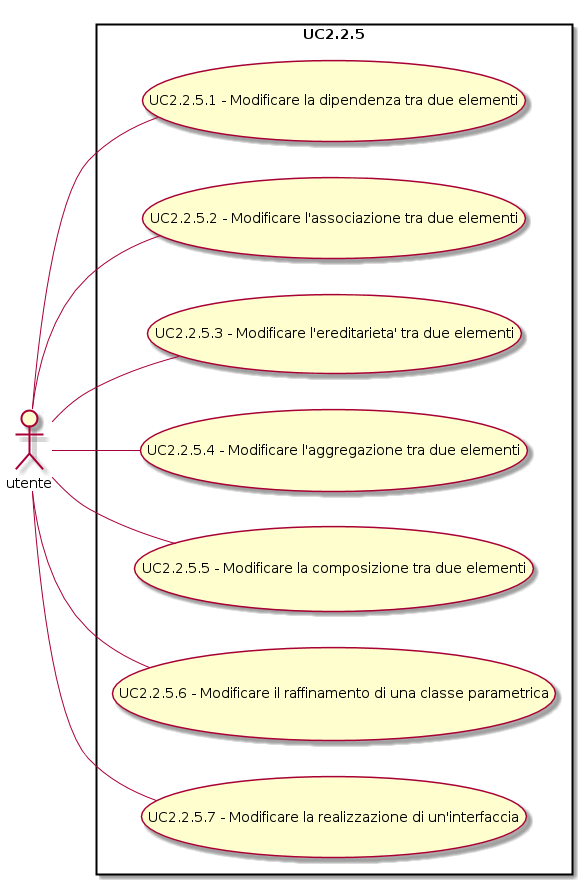
\includegraphics[scale=0.45]{./Figures/UC2-2-5.png}
				\caption{Diagramma UC2.2.5}\label{}
			\end{figure}
			\begin{itemize}
				\item \textbf{Attori}: Utente
				\item \textbf{Descrizione}: L'utente vuole modificare una relazione tra due elementi;
				\item \textbf{Precondizione}: È presente una relazione che l'utente vuole modificare;
				\item \textbf{Flusso principale degli eventi}: \begin{itemize}
					\item L'utente vuole modificare la dipendenza tra due elementi (UC2.2.5.1);
					\item L'utente vuole modificare l'associazione tra due elementi (UC2.2.5.2);
					\item L'utente vuole modificare l'ereditarietà tra due elementi (UC2.2.5.3);
					\item L'utente vuole modificare l'aggregazione tra due elementi (UC2.2.5.4);
					\item L'utente vuole modificare la composizione tra due elementi (UC2.2.5.5);
					\item L'utente vuole modificare il raffinamento di una classe parametrica (UC2.2.5.6);
					\item L'utente vuole modificare la realizzazione di un'interfaccia (UC2.2.5.7).
				\end{itemize}
				\item \textbf{Postcondizione}: .
			\end{itemize}
			\subsection{Caso d'uso UC2.2.5.1: Modificare la dipendenza tra due elementi}
			\begin{itemize}
				\item \textbf{Attori}: Utente
				\item \textbf{Descrizione}: L'utente vuole modificare la dipendenza tra due elementi;
				\item \textbf{Precondizione}: Sono presenti due elementi che hanno una relazione di dipendenza e l'utente vuole modificare questa relazione;
				\item \textbf{Flusso principale degli eventi}: L'utente modifica la dipendenza tra due elementi;
				\item \textbf{Postcondizione}: La dipendenza tra le due elementi è stata modificata.
			\end{itemize}
			\subsection{Caso d'uso UC2.2.5.2: Modificare l'associazione tra due elementi}
			\begin{itemize}
				\item \textbf{Attori}: Utente
				\item \textbf{Descrizione}: L'utente vuole modificare un'associazione tra due elementi;
				\item \textbf{Precondizione}: Sono presenti due elementi che hanno una relazione di associazione e l'utente vuole modificarne la relazione;
				\item \textbf{Flusso principale degli eventi}: L'utente modifica un'associazione tra due elementi;
				\item \textbf{Postcondizione}: L'associazione tra le due elementi è stata modificata.
			\end{itemize}
			\subsection{Caso d'uso UC2.2.5.3: Modificare l'ereditarietà tra due elementi}
			\begin{itemize}
				\item \textbf{Attori}: Utente
				\item \textbf{Descrizione}: L'utente vuole modificare una relazione di ereditarietà tra due elementi;
				\item \textbf{Precondizione}: Sono presenti due elementi che hanno una relazione di ereditarietà e l'utente vuole modificare questa relazione;
				\item \textbf{Flusso principale degli eventi}: L'utente modifica una relazione di ereditarietà tra due elementi;
				\item \textbf{Postcondizione}: L'ereditarietà tra le due elementi è stata modificata.
			\end{itemize}
			\subsection{Caso d'uso UC2.2.5.4: Modificare l'aggregazione tra due elementi}
			\begin{itemize}
				\item \textbf{Attori}: Utente
				\item \textbf{Descrizione}: L'utente vuole modificare un vincolo di aggregazione tra due elementi;
				\item \textbf{Precondizione}: Sono presenti due elementi che hanno un vinscolo di aggregazione e l'utente vuole modificare la relazione;
				\item \textbf{Flusso principale degli eventi}: L'utente modifica un vincolo di aggregazione tra due elementi;
				\item \textbf{Postcondizione}: L'aggregazione tra le due elementi è stata definita.
			\end{itemize}
			\subsection{Caso d'uso UC2.2.5.5: Modificare la composizione tra due elementi}
			\begin{itemize}
				\item \textbf{Attori}: Utente
				\item \textbf{Descrizione}: L'utente vuole modificare una composizione tra due elementi;
				\item \textbf{Precondizione}: Sono presenti due elementi con relazione di composizione e l'utente vuole modificarne la relazione;
				\item \textbf{Flusso principale degli eventi}: L'utente modifica una composizione tra due elementi;
				\item \textbf{Postcondizione}: La relazione di composizione tra i due elementi è stata definita.	
			\end{itemize}
			\subsection{Caso d'uso UC2.2.5.6: Modificare il raffinamento di una classe parametrica}
			\begin{itemize}
				\item \textbf{Attori}: Utente
				\item \textbf{Descrizione}: L'utente vuole modificare il raffinamento di una classe parametrica;
				\item \textbf{Precondizione}: L'utente si trova nella schermata dell'editor del diagramma delle classi ha selezionato il raffinamento di una classe parametrica che desidera modificare;
				\item \textbf{Flusso principale degli eventi}: L'utente modifica il raffinamento di una classe parametrica;
				\item \textbf{Postcondizione}: La relazione di raffinamento viene modificata.
			\end{itemize}
			\subsection{Caso d'uso UC2.2.5.7: Modificare la realizzazione di un'interfaccia}
			\begin{itemize}
				\item \textbf{Attori}: Utente
				\item \textbf{Descrizione}: L'utente vuole modificare la relazione di realizzazione tra un'interfaccia e una classe all'interno del diagramma delle classi;
				\item \textbf{Precondizione}: L'utente sta visualizzando il diagramma delle classi e sono presenti un'interfaccia e una classe che la realizza;
				\item \textbf{Flusso principale degli eventi}: L'utente modifica la relazione di realizzazione tra un'interfaccia e una classe all'interno del diagramma delle classi;
				\item \textbf{Postcondizione}: Nell'editor del diagramma delle classi del sistema è visualizzato il diagramma dove è stata modificatala realizzazione.
			\end{itemize}
			\subsection{Caso d'uso UC2.2.6: Eliminare una relazione}
			\begin{itemize}
				\item \textbf{Attori}: Utente
				\item \textbf{Descrizione}: L'utente vuole eliminare una relazione;
				\item \textbf{Precondizione}: Esiste una relazione che l'utente desidera eliminare;
				\item \textbf{Flusso principale degli eventi}: L'utente elimina una relazione tra due classi;
				\item \textbf{Postcondizione}: La relazione viene eliminata.
			\end{itemize}
			\subsection{Caso d'uso UC2.2.7: Creare una nuova interfaccia}
			\begin{itemize}
				\item \textbf{Attori}: Utente
				\item \textbf{Descrizione}: L'utente vuole creare un'interfaccia;
				\item \textbf{Precondizione}: Il sistema è pronto alla creazione di un'interfaccia, l'utente desidera creare un'interfaccia;
				\item \textbf{Flusso principale degli eventi}: L'utente crea un'interfaccia;
				\item \textbf{Postcondizione}: Nell'editor del diagramma delle classi l'interfaccia è correttamente visualizzato il diagramma nel quale è stata creata l'interfaccia.
			\end{itemize}
			\subsection{Caso d'uso UC2.2.8: Modificare un'interfaccia mediante la schermata di modifica dell'interfaccia}
			\begin{figure} [H]
				\centering
				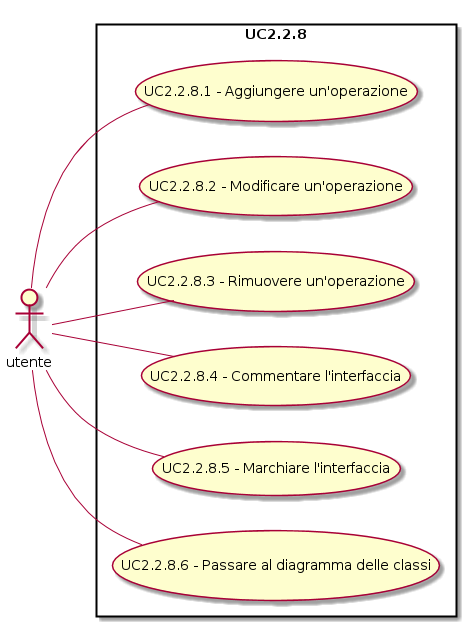
\includegraphics[scale=0.45]{./Figures/UC2-2-8.png}
				\caption{Diagramma UC2.2.8}\label{}
			\end{figure}
			\begin{itemize}
				\item \textbf{Attori}: Utente
				\item \textbf{Descrizione}: L'utente vuole modificare un'interfaccia;
				\item \textbf{Precondizione}: L'utente si trova nell'editor delle classi ed il sistema è pronto per ricevere un comando;
				\item \textbf{Flusso principale degli eventi}: \begin{itemize}
					\item L'utente può aggiungere un'operazione (UC2.2.8.1);
					\item L'utente può modificare un'operazione (UC2.2.8.2);
					\item L'utente può rimuovere un'operazione (UC2.2.8.3);
					\item L'utente può commentare l'interfaccia (UC2.2.8.4);
					\item L'utente può marchiare l'interfaccia (UC2.2.8.5);
					\item L'utente può passare dalla modifica dell'interfaccia al diagramma delle classi (UC2.2.8.6).
				\end{itemize}
				\item \textbf{Scenari alternativi}: Viene annullata la modifica, l'interfaccia rimane nello stato precedente al tentativo di modifica;
				\item \textbf{Postcondizione}: Le modifiche decise dall'utente vengono applicate all'interfaccia;
			\end{itemize}
			\subsection{Caso d'uso UC2.2.8.1: Aggiungere un'operazione}
			\begin{itemize}
				\item \textbf{Attori}: Utente
				\item \textbf{Descrizione}: L'utente vuole aggiungere un'operazione all'interfaccia;
				\item \textbf{Precondizione}: Nella schermata di modifica di interfaccia il sistema è pronto a ricevere un comando dall'utente;
				\item \textbf{Flusso principale degli eventi}: L'utente aggiunge un'operazione all'interfaccia;
				\item \textbf{Postcondizione}: Nella schermata di modifica di interfaccia è visualizzata la classe a cui è stata aggiunta l'operazione desiderata;
			\end{itemize}
			\subsection{Caso d'uso UC2.2.8.2: Modificare un'operazione}
			\begin{figure} [H]
				\centering
				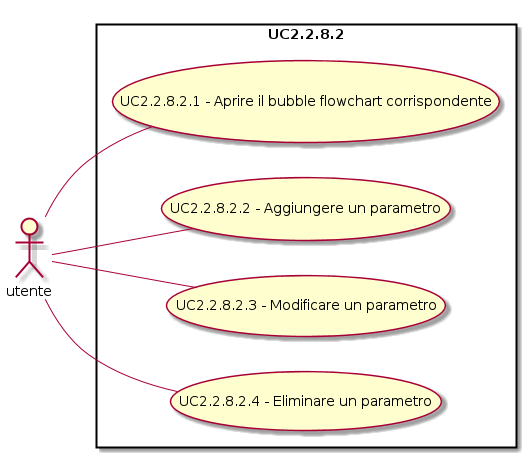
\includegraphics[scale=0.45]{./Figures/UC2-2-8-2.png}
				\caption{Diagramma UC2.2.8.2}\label{}
			\end{figure}
			\begin{itemize}
				\item \textbf{Attori}: Utente
				\item \textbf{Descrizione}: L'utente vuole modificare un'operazione già inserita in un'interfaccia;
				\item \textbf{Precondizione}: Nella schermata di modifica di interfaccia è stata selezionata l'operazione da modificare e il sistema è pronto a ricevere un comando dall'utente;
				\item \textbf{Flusso principale degli eventi}: \begin{itemize}
					\item L'utente può apportare modifiche minori;
					\item L'utente può aprire il diagramma delle attività corrispondente (UC2.2.8.2.1);
					\item L'utente può aggiungere un parametro (UC2.2.8.2.2);
					\item L'utente può modificare un parametro (UC2.2.8.2.3);
					\item L'utente può eliminare un parametro (UC2.2.8.2.4).
				\end{itemize}
				\item \textbf{Scenari alternativi}: Viene annullata la modifica, il sistema rimane nello stato precedente al tentativo di modifica;
				\item \textbf{Postcondizione}: Nella schermata di modifica di interfaccia è visualizzato il diagramma dove è stata modificata l'operazione.
			\end{itemize}
			\subsection{Caso d'uso UC2.2.8.2.1: Aprire il diagramma delle attività corrispondente}
			\begin{itemize}
				\item \textbf{Attori}: Utente
				\item \textbf{Descrizione}: L'utente vuole aprire il diagramma delle attività associato all'operazione che vuole modificare;
				\item \textbf{Precondizione}: Nella schermata di modifica di interfaccia è stata selezionata l'operazione da modificare e il sistema è pronto a ricevere un comando dall'utente;
				\item \textbf{Flusso principale degli eventi}: L'utente apre il diagramma delle attività associato all'operazione che vuole modificare;
				\item \textbf{Postcondizione}: Il sistema visualizza il diagramma delle attività corrispondente all'operazione che l'utente vuole modificare;
			\end{itemize}
			\subsection{Caso d'uso UC2.2.8.2.2: Aggiungere un parametro}
			\begin{itemize}
				\item \textbf{Attori}: Utente
				\item \textbf{Descrizione}: L'utente vuole aggiungere un parametro alla lista parametri dell'operazione;
				\item \textbf{Precondizione}: Nella schermata di modifica di interfaccia è stata selezionata l'operazione da modificare e il sistema è pronto a ricevere un comando dall'utente;
				\item \textbf{Flusso principale degli eventi}: L'utente aggiunge un parametro alla lista parametri dell'operazione;
				\item \textbf{Postcondizione}: Nella schermata di modifica di interfaccia è visualizzato il diagramma dove è stato aggiunto un parametro alla lista parametri dell'operazione.
			\end{itemize}
			\subsection{Caso d'uso UC2.2.8.2.3: Modificare un parametro}
			\begin{itemize}
				\item \textbf{Attori}: Utente
				\item \textbf{Descrizione}: L'utente vuole modificare un parametro della lista parametri dell'operazione;
				\item \textbf{Precondizione}: Nella schermata di modifica di interfaccia è stata selezionata l'operazione da modificare e il sistema è pronto a ricevere un comando dall'utente;
				\item \textbf{Flusso principale degli eventi}: L'utente modifica il parametro;
				\item \textbf{Scenari alternativi}: Viene annullata la modifica, il parametro rimane nello stato precedente al tentativo di modifica;
				\item \textbf{Postcondizione}: Nella schermata di modifica di interfaccia è visualizzato il diagramma dove è stato modificato un parametro nella lista parametri dell'operazione.
			\end{itemize}
			\subsection{Caso d'uso UC2.2.8.2.4: Eliminare un parametro}
			\begin{itemize}
				\item \textbf{Attori}: Utente
				\item \textbf{Descrizione}: L'utente vuole eliminare un parametro;
				\item \textbf{Precondizione}: Nella schermata di modifica di interfaccia è stata selezionato il parametro da rimuovere e il sistema è pronto a ricevere un comando dall'utente;
				\item \textbf{Flusso principale degli eventi}: L'utente elimina un parametro;
				\item \textbf{Postcondizione}: Nella schermata di modifica di interfaccia è visualizzato il diagramma dove è stato rimosso il parametro dalla lista parametri dell'operazione.	
			\end{itemize}
			\subsection{Caso d'uso UC2.2.8.3: Rimuovere un'operazione}
			\begin{itemize}
				\item \textbf{Attori}: Utente
				\item \textbf{Descrizione}: L'utente vuole rimuovere un'operazione;
				\item \textbf{Precondizione}: Nella schermata di modifica di interfaccia è stata selezionata l'operazione da rimuovere e il sistema è pronto a ricevere un comando dall'utente;
				\item \textbf{Flusso principale degli eventi}: L'utente rimuove l'operazione;
				\item \textbf{Postcondizione}: Nella schermata di modifica di interfaccia è visualizzato il diagramma dove è stata rimossa l'operazione.
			\end{itemize}
			\subsection{Caso d'uso UC2.2.8.4: Commentare l'interfaccia}
			\begin{itemize}
				\item \textbf{Attori}: Utente
				\item \textbf{Descrizione}: L'utente vuole commentare l'interfaccia;
				\item \textbf{Precondizione}: Nella schermata di modifica di interfaccia è stata selezionata l'interfaccia da commentare e il sistema è pronto a ricevere un comando dall'utente;
				\item \textbf{Flusso principale degli eventi}: L'utente commenta l'interfaccia;
				\item \textbf{Postcondizione}: Nella schermata di modifica di interfaccia è visualizzato il diagramma dove è stata commentata l'interfaccia.
			\end{itemize}
			\subsection{Caso d'uso UC2.2.8.5: Marchiare l'interfaccia}
			\begin{itemize}
				\item \textbf{Attori}: Utente
				\item \textbf{Descrizione}: L'utente vuole marchiare l'interfaccia;
				\item \textbf{Precondizione}: Nella schermata di modifica di interfaccia è stata selezionata l'interfaccia da marchiare e il sistema è pronto a ricevere un comando dall'utente;
				\item \textbf{Flusso principale degli eventi}: L'utente marchia l'interfaccia;
				\item \textbf{Postcondizione}: Nella schermata di modifica di interfaccia è visualizzato il diagramma dove è stata marchiata l'interfaccia.
			\end{itemize}
			\subsection{Caso d'uso UC2.2.8.6: Passare dalla modifica di interfaccia al diagramma delle classi}
			\begin{itemize}
				\item \textbf{Attori}: Utente
				\item \textbf{Descrizione}: L'utente vuole tornare al diagramma delle classi dalla schermata di modifica di interfaccia;
				\item \textbf{Precondizione}: Il sistema visualizza la schermata di modifica di interfaccia;
				\item \textbf{Flusso principale degli eventi}: L'utente torna al diagramma delle classi dalla schermata di modifica di interfaccia;
				\item \textbf{Postcondizione}: Il sistema visualizza l'editor del diagramma delle classi
			\end{itemize}
			\subsection{Caso d'uso UC2.2.9: Eliminare un'interfaccia}
			\begin{itemize}
				\item \textbf{Attori}: Utente
				\item \textbf{Descrizione}: L'utente vuole eliminare un'interfaccia dal diagramma delle classi;
				\item \textbf{Precondizione}: L'utente ha selezionato l'interfaccia che vuole rimuovere;
				\item \textbf{Flusso principale degli eventi}: L'utente elimina un'interfaccia dal diagramma delle classi;
				\item \textbf{Postcondizione}: Nell'editor del diagramma delle classi è visualizzato il diagramma dove è stata rimossa l'interfaccia.
			\end{itemize}
			\subsection{Caso d'uso UC2.2.10: Creare un commento}
			\begin{itemize}
				\item \textbf{Attori}: Utente
				\item \textbf{Descrizione}: L'utente vuole creare commento all'interno del diagramma delle classi;
				\item \textbf{Precondizione}: L'utente ha avviato il programma aperto nel diagramma delle classi;
				\item \textbf{Flusso principale degli eventi}: L'utente crea un commento all'interno del diagramma delle classi;
				\item \textbf{Postcondizione}: Il commento viene aggiunto al diagramma delle classi;
			\end{itemize}
			\subsection{Caso d'uso UC2.2.11: Collegare un commento}
			\begin{itemize}
				\item \textbf{Attori}: Utente
				\item \textbf{Descrizione}: L'utente vuole collegare un commento a un altro elemento;
				\item \textbf{Precondizione}: L'utente ha avviato il programma e ha il diagramma delle classi aperto;
				\item \textbf{Flusso principale degli eventi}: L'utente collega un commento a un altro elemento;
				\item \textbf{Postcondizione}: Il commento viene collegato all'elemento nel diagramma delle classi.
			\end{itemize}
			\subsection{Caso d'uso UC2.2.12: Modificare un commento}
			\begin{itemize}
				\item \textbf{Attori}: Utente
				\item \textbf{Descrizione}: L'utente vuole modificare un commento nel diagramma delle classi;
				\item \textbf{Precondizione}: L'utente ha selezioneto il commento che cuole modificare all'interno del diagramma delle classi;
				\item \textbf{Flusso principale degli eventi}: L'utente modifica un commento nel diagramma delle classi;
				\item \textbf{Postcondizione}: Il commento all'interno del diagramma delle classi viene modificato.
			\end{itemize}
			\subsection{Caso d'uso UC2.2.13: Eliminare un commento}
			\begin{itemize}
				\item \textbf{Attori}: Utente
				\item \textbf{Descrizione}: L'utente vuole eliminare un commento dal diagramma delle classi;
				\item \textbf{Precondizione}: L'utente ha selezionato il commento che vuole eliminare;
				\item \textbf{Flusso principale degli eventi}: L'utente elimina un commento dal diagramma delle classi;
				\item \textbf{Postcondizione}: Il commento viene eliminato dal diagramma delle classi.
			\end{itemize}
			\subsection{Caso d'uso UC2.2.14: Modificare una classe mediante la schermata di modifica di una classe}
			\begin{figure} [H]
				\centering
				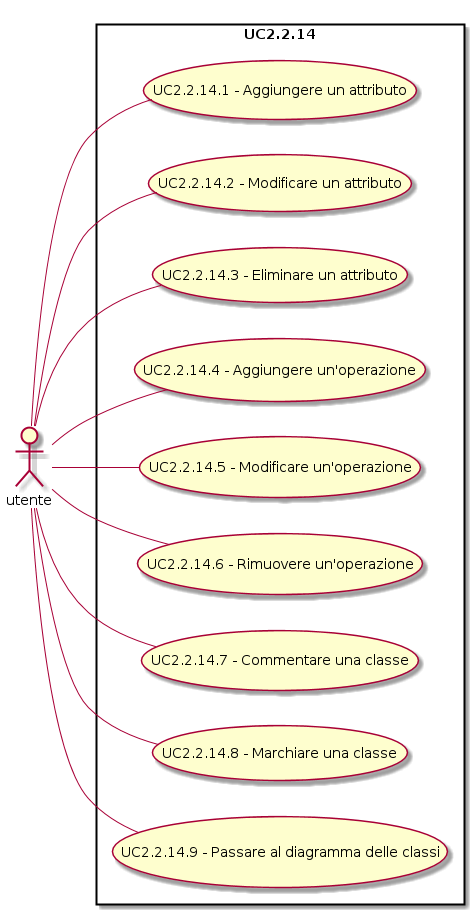
\includegraphics[scale=0.45]{./Figures/UC2-2-14.png}
				\caption{Diagramma UC2.2.14}\label{}
			\end{figure}
			\begin{itemize}
				\item \textbf{Attori}: Utente
				\item \textbf{Descrizione}: L'utente vuole modificare una classe;
				\item \textbf{Precondizione}: L'utente ha selezionato una classe all'interno del diagramma delle classi che vuole modificare;
				\item \textbf{Flusso principale degli eventi}: \begin{itemize}
					\item L'utente può aggiungere un attributo (UC2.2.14.1);
					\item L'utente può modificare un attributo (UC2.2.14.2);
					\item L'utente può eliminare un attributo (UC2.2.14.3);
					\item L'utente può aggiungere un'operazione (UC2.2.14.4);
					\item L'utente può modificare un'operazione (UC2.2.14.5);
					\item L'utente può rimuovere un'operazione (UC2.2.14.6);
					\item L'utente può commentare una classe (UC2.2.14.7);
					\item L'utente può marchiare una classe (UC2.2.14.8);
					\item L'utente può tornare al diagramma delle classi (UC2.2.14.9).
				\end{itemize}
				\item \textbf{Scenari alternativi}: Viene annullata la modifica, la classe rimane nello stato precedente al tentativo di modifica;
				\item \textbf{Postcondizione}: Le modifiche decise dall'utente vengono applicate alla classe.
			\end{itemize}
			\subsection{Caso d'uso UC2.2.14.1: Aggiungere un attributo}
			\begin{itemize}
				\item \textbf{Attori}: Utente
				\item \textbf{Descrizione}: L'utente vuole aggiungere un attributo ad una classe;
				\item \textbf{Precondizione}: L'utente ha selezionato una classe all'interno del diagramma delle classi alla quale vuole aggiungere un attributo;
				\item \textbf{Flusso principale degli eventi}: L'utente aggiunge un attributo alla classe e da un valore al tipo, al nome e un eventuale valore di default dell'attributo. 
				\item \textbf{Scenari alternativi}: Viene annullata la modifica, la classe rimane nello stato precedente al tentativo di aggiunta;
				\item \textbf{Postcondizione}: L'attributo viene aggiunto alla classe con i parametri decisi dall'utente.
			\end{itemize}
			\subsection{Caso d'uso UC2.2.14.2: Modificare un attributo}
			\begin{itemize}
				\item \textbf{Attori}: Utente
				\item \textbf{Descrizione}: L'utente vuole modificare un attributo di una classe;
				\item \textbf{Precondizione}: L'utente ha selezionato l'attributo che vuole modificare all'interno di una classe;
				\item \textbf{Flusso principale degli eventi}: L'utente modifica l'attributo della classe;
				\item \textbf{Scenari alternativi}: Viene annullata la modifica, il campo dati rimane nello stato precedente al tentativo di modifica;
				\item \textbf{Postcondizione}: Le modifiche decise dall'utente vengono applicate all'attributo all'interno della classe.
			\end{itemize}
			\subsection{Caso d'uso UC2.2.14.3: Eliminare un attributo}
			\begin{itemize}
				\item \textbf{Attori}: Utente
				\item \textbf{Descrizione}: L'utente vuole eliminare un attributo all'interno di una classe;
				\item \textbf{Precondizione}: L'utente ha selezionato l'attributo che vuole eliminare;
				\item \textbf{Flusso principale degli eventi}: L'utente elimina un attributo;
				\item \textbf{Scenari alternativi}: Viene annullata la modifica, la classe rimane nello stato precedente al tentativo di eliminazione;
				\item \textbf{Postcondizione}: L'attributo viene eliminato dalla classe dopo eventuali avvisi nel caso ci siano dipendenze da controllare.
			\end{itemize}
			\subsection{Caso d'uso UC2.2.14.4: Aggiungere un'operazione}
			\begin{itemize}
				\item \textbf{Attori}: Utente
				\item \textbf{Descrizione}: L'utente vuole aggiungere un'operazione ad una classe;
				\item \textbf{Precondizione}: L'utente ha selezionato una classe all'interno del diagramma delle classi alla quale vuole aggiungere un'operazione;
				\item \textbf{Flusso principale degli eventi}: L'utente aggiunge un'operazione ad una classe;
				\item \textbf{Scenari alternativi}: Viene annullata la modifica, la classe rimane nello stato precedente al tentativo di aggiunta;
				\item \textbf{Postcondizione}: L'operazione viene aggiunta alla classe con i parametri decisi dall'utente.
			\end{itemize}
			\subsection{Caso d'uso UC2.2.14.5: Modificare un'operazione}
			\begin{figure} [H]
				\centering
				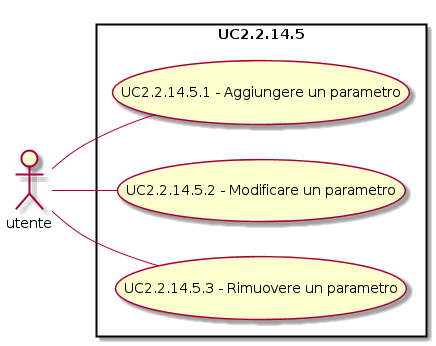
\includegraphics[scale=0.45]{./Figures/UC2-2-14-5.png}
				\caption{Diagramma UC2.2.14.5}\label{}
			\end{figure}
			\begin{itemize}
				\item \textbf{Attori}: Utente
				\item \textbf{Descrizione}: L'utente vuole modificare un' operazione all'interno di una classe;
				\item \textbf{Precondizione}: L'utente ha selezionato l'operazione che vuole modificare all'interno di una classe;
				\item \textbf{Flusso principale degli eventi}: \begin{itemize}
					\item L'utente può aggiungere un parametro (UC2.2.14.5.1);
					\item L'utente può modificare un parametro (UC2.2.14.5.2);
					\item L'utente può eliminare un parametro (UC2.2.14.5.3);
					\item L'utente può apportare modifiche minori.
				\end{itemize}
				\item \textbf{Scenari alternativi}: Viene annullata la modifica, l'operazione rimane nello stato precedente al tentativo di modifica;
				\item \textbf{Postcondizione}: Le modifiche decise dall'utente vengono applicate all'operazione all'interno della classe.
			\end{itemize}
			\subsection{Caso d'uso UC2.2.14.5.1: Aggiungere un parametro}
			\begin{itemize}
				\item \textbf{Attori}: Utente
				\item \textbf{Descrizione}: L'utente vuole aggiungere un parametro alla lista parametri dell'operazione;
				\item \textbf{Precondizione}: Nella schermata di modifica delle classi è stata selezionata l'operazione da modificare e il sistema è pronto a ricevere un comando dall'utente;
				\item \textbf{Flusso principale degli eventi}: L'utente aggiunge un parametro alla lista parametri dell'operazione;
				\item \textbf{Postcondizione}: Nella schermata di modifica delle classi è visualizzato il parametro che è stato aggiunto alla lista parametri dell'operazione.
			\end{itemize}
			\subsection{Caso d'uso UC2.2.14.5.2: Modificare un parametro}
			\begin{itemize}
				\item \textbf{Attori}: Utente
				\item \textbf{Descrizione}: L'utente vuole modificare un parametro della lista parametri dell'operazione;
				\item \textbf{Precondizione}: Nella schermata di modifica delle classi è stata selezionata l'operazione da modificare e il sistema è pronto a ricevere un comando dall'utente;
				\item \textbf{Flusso principale degli eventi}: \begin{itemize} \item L'utente può definire la direzione del parametro; \item L'utente può rinominare il parametro; \item L'utente può definire il tipo del parametro; \item L'utente può definire il valore di default del parametro. \end{itemize}
				\item \textbf{Postcondizione}: Nella schermata di modifica delle classi è visualizzato il parametro che è stato modificato nella lista parametri dell'operazione.
			\end{itemize}
			\subsection{Caso d'uso UC2.2.14.5.3: Rimuovere un parametro}
			\begin{itemize}
				\item \textbf{Attori}: Utente
				\item \textbf{Descrizione}: L'utente vuole rimuovere un parametro;
				\item \textbf{Precondizione}: Nella schermata di modifica delle classi è stata selezionata l'operazione da modificare e il sistema è pronto a ricevere un comando dall'utente;
				\item \textbf{Flusso principale degli eventi}: L'utente rimuove un parametro;
				\item \textbf{Postcondizione}: Nella schermata di modifica delle classi è visualizzato il parametro che è stato rimosso dalla lista parametri dell'operazione.
			\end{itemize}
			\subsection{Caso d'uso UC2.2.14.6: Rimuovere un'operazione}
			\begin{itemize}
				\item \textbf{Attori}: Utente
				\item \textbf{Descrizione}: L'utente vuole rimuovere un'operazione all'interno di una classe;
				\item \textbf{Precondizione}: L'utente ha selezionato l'operazione che vuole rimuovere;
				\item \textbf{Flusso principale degli eventi}: L'utente rimuove un'operazione all'interno di una classe;
				\item \textbf{Scenari alternativi}: Viene annullata la modifica, la classe rimane nello stato precedente al tentativo di rimozione;
				\item \textbf{Postcondizione}: L'operazione viene rimossa dalla classe dopo eventuali avvisi nel caso ci siano dipendenze da controllare.
			\end{itemize}
			\subsection{Caso d'uso UC2.2.14.7: Commentare una classe}
			\begin{itemize}
				\item \textbf{Attori}: Utente
				\item \textbf{Descrizione}: L'utente vuole commentare una classe;
				\item \textbf{Precondizione}: L'utente ha selezionato la classe che desidera commentare;
				\item \textbf{Flusso principale degli eventi}: L'utente commenta una classe;
				\item \textbf{Scenari alternativi}: Viene annullata la modifica, la classe rimane nello stato precedente al tentativo di modifica;
				\item \textbf{Postcondizione}: Il commento relativo alla classe viene impostato.
			\end{itemize}
			\subsection{Caso d'uso UC2.2.14.8: Marchiare una classe}
			\begin{itemize}
				\item \textbf{Attori}: Utente
				\item \textbf{Descrizione}: L'utente vuole marchiare una classe con un attributo;
				\item \textbf{Precondizione}: L'utente ha selezionato la classe che desidera marchiare;
				\item \textbf{Flusso principale degli eventi}: L'utente marchia una classe con un attributo;
				\item \textbf{Scenari alternativi}: Viene annullata la modifica, la classe rimane nello stato precedente al tentativo di modifica;
				\item \textbf{Postcondizione}: La classe è stata marchiata con un attributo.
			\end{itemize}
			\subsection{Caso d'uso UC2.2.14.9: Passare dalla modifica di una classe al diagramma delle classi}
			\begin{itemize}
				\item \textbf{Attori}: Utente
				\item \textbf{Descrizione}: L'utente vuole spostarsi nella schermata del diagramma delle classi;
				\item \textbf{Precondizione}: L'utente si trova nella schermata di modifica delle classi;
				\item \textbf{Flusso principale degli eventi}: L'utente si sposta nella schermata del diagramma delle classi;
				\item \textbf{Postcondizione}: L'utente si trova nella schermata del diagramma delle classi.
			\end{itemize}
			\subsection{Caso d'uso UC2.2.15: Riposizionare un elemento}
			\begin{itemize}
				\item \textbf{Attori}: Utente
				\item \textbf{Descrizione}: L'utente vuole cambiare la posizione di un elemento all'interno del diagramma;
				\item \textbf{Precondizione}: L'utente si trova nella schermata dell'editor del diagramma delle classi e il sistema è pronto a ricevere un comando dall'utente;
				\item \textbf{Flusso principale degli eventi}: L'utente riposiziona l'elemento;
				\item \textbf{Postcondizione}: Il sistema visualizza il diagramma con l'elemento riposizionato correttamente;
			\end{itemize}
			\subsection{Caso d'uso UC2.3: Editare il diagramma delle attività}
				\begin{figure} [H]
					\centering
					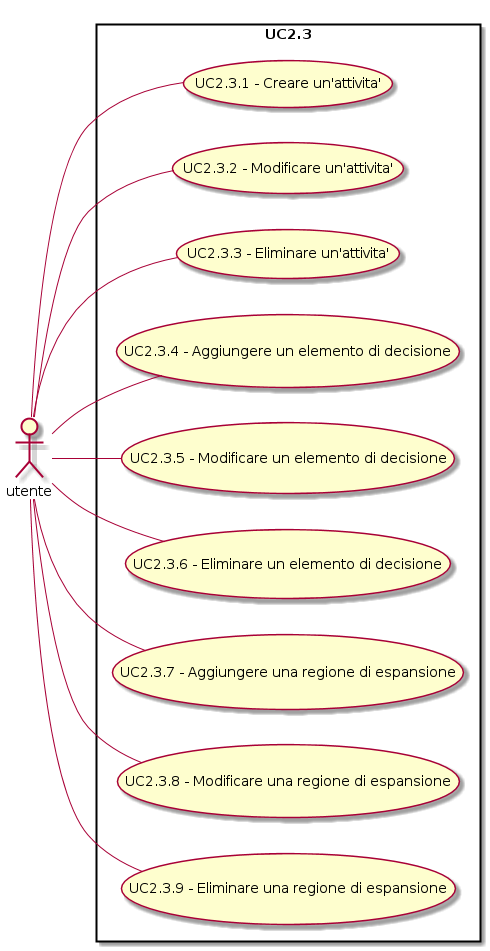
\includegraphics[scale=0.45]{./Figures/UC2-3parte1.png}
					\caption{Diagramma UC2.3 prima parte}\label{}
				\end{figure}
				\begin{figure} [H]
					\centering
					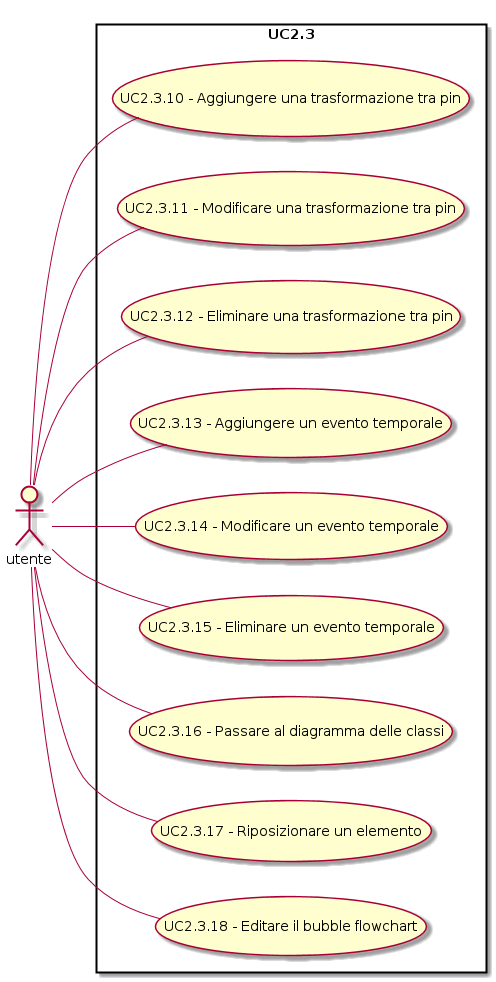
\includegraphics[scale=0.45]{./Figures/UC2-3parte2.png}
					\caption{Diagramma UC2.3 seconda parte}\label{}
				\end{figure}
				\begin{itemize}
					\item \textbf{Attori}: Utente
					\item \textbf{Descrizione}: L'utente vuole editare il diagramma delle attività;
					\item \textbf{Precondizione}: L'utente si trova nella schermata dell'editor del diagramma delle attività e il sistema è pronto a ricevere un comando dall'utente;
					\item \textbf{Flusso principale degli eventi}: \begin{itemize}
						\item L'utente può creare un'attività (UC2.3.1);
						\item L'utente può modificare un'attività (UC2.3.2);
						\item L'utente può eliminare un'attività (UC2.3.3);
						\item L'utente può aggiungere un elemento di decisione (UC2.3.4);
						\item L'utente può modificare un elemento di decisione (UC2.3.5);
						\item L'utente può eliminare un elemento di decisione (UC2.3.6);
						\item L'utente può aggiungere una regione di espansione (UC2.3.7);
						\item L'utente può modificare una regione di espansione (UC2.3.8);
						\item L'utente può eliminare una regione di espansione (UC2.3.9);
						\item L'utente può aggiungere una trasformazione tra pin (UC2.3.10);
						\item L'utente può modificare una trasformazione tra pin (UC2.3.11);
						\item L'utente può rimuovere una trasformazione tra pin (UC2.3.12);
						\item L'utente può aggiungere un evento temporale (UC2.3.13);
						\item L'utente può modificare un evento temporale (UC2.3.14);
						\item L'utente può rimuovere un evento temporale (UC2.3.15);
						\item L'utente può passare dal diagramma delle attività al diagramma delle classi (UC2.3.16);
						\item L'utente può riposizionare un elemento (UC2.3.17);
						\item L'utente può editare il Bubble Flowchart (UC2.3.18).
					\end{itemize}
					\item \textbf{Scenari alternativi}: Viene annullata la modifica, l'interfaccia rimane nello stato precedente al tentativo di modifica;
					\item \textbf{Postcondizione}: Nella schermata dell'editor del diagramma delle attività è mostrato il diagramma come è stato editato dall'utente e il sistema è pronto a ricevere un nuovo comando.
				\end{itemize}
				\subsection{Caso d'uso UC2.3.1: Creare un'attività}
				\begin{itemize}
					\item \textbf{Attori}: Utente
					\item \textbf{Descrizione}: L'utente vuole creare un'attività;
					\item \textbf{Precondizione}: L'utente si trova nella schermata dell'editor del diagramma delle attività e il sistema è pronto a ricevere un comando dall'utente;
					\item \textbf{Flusso principale degli eventi}: L'utente crea una nuova attività che viene aggiunta nel diagramma delle attività.
					\item \textbf{Postcondizione}: Nella schermata dell'editor del diagramma delle attività è visualizzato il diagramma a cui è stata aggiunta la nuova attività.
				\end{itemize}
				\subsection{Caso d'uso UC2.3.2: Modificare un'attività}
				\begin{figure} [H]
					\centering
					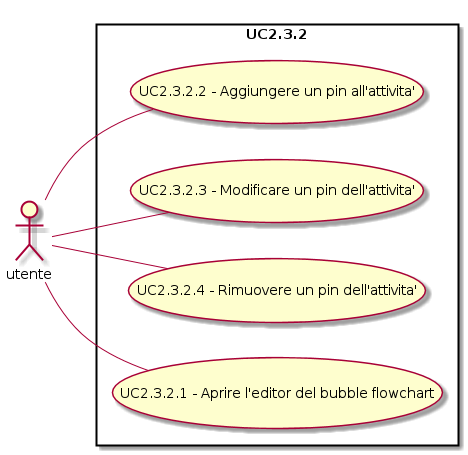
\includegraphics[scale=0.45]{./Figures/UC2-3-2.png}
					\caption{Diagramma UC2.3.2}\label{}
				\end{figure}
				\begin{itemize}
					\item \textbf{Attori}: Utente
					\item \textbf{Descrizione}: L'utente vuole modificare un'attività;
					\item \textbf{Precondizione}: Nella schermata dell'editor del diagramma delle attività è stata selezionata l'attività da modificare e il sistema è pronto a ricevere un comando dall'utente;
					\item \textbf{Flusso principale degli eventi}: \begin{itemize}
						\item L'utente può apportare modifiche minori;
						\item L'utente può aprire l'editor del bubble flowchart (UC2.3.2.1);
						\item L'utente può aggiungere un pin all'attività (UC2.3.2.2);
						\item L'utente può modificare un pin dell'attività (UC2.3.2.3);
						\item L'utente può rimuovere un pin dell'attività (UC2.3.2.4);
					\end{itemize}
					\item \textbf{Scenari alternativi}: Viene annullata la modifica, il sistema rimane nello stato precedente al tentativo di modifica;
					\item \textbf{Postcondizione}: Nella schermata dell'editor del diagramma delle attività è visualizzato il diagramma in cui è stata modificata l'attività.
				\end{itemize}
				\subsection{Caso d'uso UC2.3.2.1: Aprire l'editor del bubble flowchart}
				\begin{itemize}
					\item \textbf{Attori}: Utente
					\item \textbf{Descrizione}: L'utente vuole aprire l'editor del bubble flowchart; 
					\item \textbf{Precondizione}: Nella schermata dell'editor del diagramma delle attività è stata selezionata l'attività di cui si vuole editare il bubble flowchart e il sistema è pronto a ricevere un comando dall'utente;
					\item \textbf{Flusso principale degli eventi}: L'utente apre l'editor del bubble flowchart;
					\item \textbf{Postcondizione}: Il sistema visualizza la schermata dell'editor del bubble flowchart con aperto il diagramma della attività corrispondente. Il sistema è pronto a ricevere un nuovo comando dall'utente.
				\end{itemize}
				\subsection{Caso d'uso UC2.3.2.2: Aggiungere un pin all'attività}
				\begin{itemize}
					\item \textbf{Attori}: Utente
					\item \textbf{Descrizione}: L'utente vuole aggiungere un pin all'attività;
					\item \textbf{Precondizione}: Nella schermata dell'editor del diagramma delle attività è stata selezionata l'attività a cui aggiungere un pin e il sistema è pronto a ricevere un comando dall'utente;
					\item \textbf{Flusso principale degli eventi}: L'utente aggiunge un pin all'attività;
					\item \textbf{Postcondizione}: Nella schermata dell'editor del diagramma delle attività è visualizzato il diagramma in cui è stato aggiunto il pin all'attività.
				\end{itemize}
				\subsection{Caso d'uso UC2.3.2.3: Modificare un pin dell'attività}
				\begin{itemize}
					\item \textbf{Attori}: Utente
					\item \textbf{Descrizione}: L'utente vuole modificare un pin dell'attività;
					\item \textbf{Precondizione}: Nella schermata dell'editor del diagramma delle attività è stato selezionato il pin da modificare e il sistema è pronto a ricevere un comando dall'utente;
					\item \textbf{Flusso principale degli eventi}: \begin{itemize}
						\item L'utente può definire la direzione del parametro corrispondente;
						\item L'utente può rinominare il parametro corrispondente;
						\item L'utente può definire il tipo del parametro corrispondente;
						\item L'utente può definire il valore di default del parametro corrispondente;
					\end{itemize}
						\item \textbf{Scenari alternativi}: Viene annullata la modifica, il sistema rimane nello stato precedente al tentativo di modifica;
						\item \textbf{Postcondizione}: Nella schermata dell'editor del diagramma delle attività è visualizzato il diagramma in cui è stato modificato il pin dell'attività.
					\end{itemize}
					\subsection{Caso d'uso UC2.3.2.4: Rimuovere un pin dell'attività}
					\begin{itemize}
						\item \textbf{Attori}: Utente
						\item \textbf{Descrizione}: L'utente vuole rimuovere un pin dell'attività;
						\item \textbf{Precondizione}: Nella schermata dell'editor del diagramma delle attività è stato selezionato il pin da rimuovere e il sistema è pronto a ricevere un comando dall'utente;
						\item \textbf{Flusso principale degli eventi}: L'utente rimuove il pin selezionato dal diagramma delle attività;
						\item \textbf{Postcondizione}: Nella schermata dell'editor del diagramma delle attività è visualizzato il diagramma in cui è stato rimosso il pin all'attività.
					\end{itemize}
					\subsection{Caso d'uso UC2.3.3: Eliminare un'attività}
					\begin{itemize}
						\item \textbf{Attori}: Utente
						\item \textbf{Descrizione}: L'utente vuole eliminare un'attività;
						\item \textbf{Precondizione}: Nella schermata dell'editor del diagramma delle attività è stata selezionata l'attività da eliminare e il sistema è pronto a ricevere un comando dall'utente;
						\item \textbf{Flusso principale degli eventi}: L'utente elimina un'attività;
						\item \textbf{Postcondizione}: Nella schermata dell'editor del diagramma delle attività è visualizzato il diagramma da cui è stata rimossa l'attività.
					\end{itemize}
					\subsection{Caso d'uso UC2.3.4: Aggiungere un elemento di decisione}
					\begin{itemize}
						\item \textbf{Attori}: Utente
						\item \textbf{Descrizione}: L'utente vuole aggiungere un elemento di decisione;
						\item \textbf{Precondizione}: L'utente si trova nella schermata dell'editor del diagramma delle attività e il sistema è pronto a ricevere un comando dall'utente;
						\item \textbf{Flusso principale degli eventi}: L'utente aggiunge un elemento di decisione, il quale viene visualizzato nel diagramma delle attività;
						\item \textbf{Postcondizione}: Nella schermata dell'editor del diagramma delle attività è visualizzato il diagramma a cui è stato aggiunto l'elemento di decisione.
					\end{itemize}
					\subsection{Caso d'uso UC2.3.5: Modificare un elemento di decisione}
					\begin{itemize}
						\item \textbf{Attori}: Utente
						\item \textbf{Descrizione}: L'utente vuole modificare un elemento di decisione;
						\item \textbf{Precondizione}: Nella schermata dell'editor del diagramma delle attività è stato selezionato l'elemento di decisione da modificare e il sistema è pronto a ricevere un comando dall'utente;
						\item \textbf{Flusso principale degli eventi}: L'utente modifica l'elemento di decisione selezionato nel diagramma delle attività;
						\item \textbf{Postcondizione}: Nella schermata dell'editor del diagramma delle attività è visualizzato il diagramma in cui è stato modificato l'elemento di decisione.
					\end{itemize}
					\subsection{Caso d'uso UC2.3.6: Eliminare un elemento di decisione}
					\begin{itemize}
						\item \textbf{Attori}: Utente
						\item \textbf{Descrizione}: L'utente vuole eliminare un elemento di decisione;
						\item \textbf{Precondizione}: Nella schermata dell'editor del diagramma delle attività è stato selezionato l'elemento di decisione da eliminare e il sistema è pronto a ricevere un comando dall'utente;
						\item \textbf{Flusso principale degli eventi}: L'utente elimina un elemento di decisione;
						\item \textbf{Postcondizione}: Nella schermata dell'editor del diagramma delle attività è visualizzato il diagramma da cui è stato rimosso l'elemento di decisione.
					\end{itemize}
					\subsection{Caso d'uso UC2.3.7: Aggiungere una regione di espansione}
					\begin{itemize}
						\item \textbf{Attori}: Utente
						\item \textbf{Descrizione}: L'utente vuole aggiungere una regione di espansione;
						\item \textbf{Precondizione}: L'utente si trova nella schermata dell'editor del diagramma delle attività e il sistema è pronto a ricevere un comando dall'utente;
						\item \textbf{Flusso principale degli eventi}: L'utente aggiunge una regione di espansione;
						\item \textbf{Postcondizione}: Nella schermata dell'editor del diagramma delle attività è visualizzato il diagramma a cui è stata aggiunta la regione di espansione;
					\end{itemize}
					\subsection{Caso d'uso UC2.3.8: Modificare una regione di espansione}
					\begin{itemize}
						\item \textbf{Attori}: Utente
						\item \textbf{Descrizione}: L'utente vuole modificare una regione di espansione;
						\item \textbf{Precondizione}: Nella schermata dell'editor del diagramma delle attività è stata selezionata la regione di espansione da modificare e il sistema è pronto a ricevere un comando dall'utente;
						\item \textbf{Flusso principale degli eventi}: L'utente modifica la regione di espansione;
						\item \textbf{Scenari alternativi}: Viene annullata la modifica, il sistema rimane nello stato precedente al tentativo di modifica;
						\item \textbf{Postcondizione}: Nella schermata dell'editor del diagramma delle attività è visualizzato il diagramma in cui è stata modificata la regione di espansione.
					\end{itemize}
					\subsection{Caso d'uso UC2.3.9: Eliminare una regione di espansione}
					\begin{itemize}
						\item \textbf{Attori}: Utente
						\item \textbf{Descrizione}: L'utente vuole eliminare una regione di espansione;
						\item \textbf{Precondizione}: Nella schermata dell'editor del diagramma delle attività è stata selezionata la regione di espansione da eliminare e il sistema è pronto a ricevere un comando dall'utente;
						\item \textbf{Flusso principale degli eventi}: L'utente elimina una regione di espansione;
						\item \textbf{Postcondizione}: Nella schermata dell'editor del diagramma delle attività è visualizzato il diagramma da cui è stata rimossa la regione di espansione.
					\end{itemize}
					\subsection{Caso d'uso UC2.3.10: Aggiungere una trasformazione tra pin}
					\begin{itemize}
						\item \textbf{Attori}: Utente
						\item \textbf{Descrizione}: L'utente vuole aggiungere una trasformazione tra pin;
						\item \textbf{Precondizione}: Nella schermata dell'editor del diagramma delle attività è stato selezionato il pin da cui far partire la trasformazione e il sistema è pronto a ricevere un comando dall'utente;
						\item \textbf{Flusso principale degli eventi}: L'utente aggiunge una trasformazione tra pin;
						\item \textbf{Postcondizione}: Nella schermata dell'editor del diagramma delle attività è visualizzato il diagramma a cui è stata aggiunta la trasformazione tra pin.
					\end{itemize}
					\subsection{Caso d'uso UC2.3.11: Modificare una trasformazione tra pin}
					\begin{itemize}
						\item \textbf{Attori}: Utente
						\item \textbf{Descrizione}: L'utente vuole modificare una trasformazione tra pin;
						\item \textbf{Precondizione}: Nella schermata dell'editor del diagramma delle attività è stata selezionata la trasformazione da modificare e il sistema è pronto a ricevere un comando dall'utente;
						\item \textbf{Flusso principale degli eventi}: L'utente modifica una trasformazione tra pin;
						\item \textbf{Scenari alternativi}: Viene annullata la modifica, il sistema rimane nello stato precedente al tentativo di modifica;
						\item \textbf{Postcondizione}: Nella schermata dell'editor del diagramma delle attività è visualizzato il diagramma in cui è stata modificata la trasformazione tra pin.
					\end{itemize}
					\subsection{Caso d'uso UC2.3.12: Eliminare una trasformazione tra pin}
					\begin{itemize}
						\item \textbf{Attori}: Utente
						\item \textbf{Descrizione}: L'utente vuole eliminare una trasformazione tra pin;
						\item \textbf{Precondizione}: Nella schermata dell'editor del diagramma delle attività è stata selezionata la trasformazione da eliminare e il sistema è pronto a ricevere un comando dall'utente;
						\item \textbf{Flusso principale degli eventi}: L'utente elimina una trasformazione tra pin;
						\item \textbf{Postcondizione}: Nella schermata dell'editor del diagramma delle attività è visualizzato il diagramma da cui è stata rimossa la trasformazione tra pin.
					\end{itemize}
					\subsection{Caso d'uso UC2.3.13: Aggiungere un evento temporale}
					\begin{itemize}
						\item \textbf{Attori}: Utente
						\item \textbf{Descrizione}: L'utente vuole aggiungere un evento temporale;
						\item \textbf{Precondizione}: L'utente si trova nella schermata dell'editor del diagramma delle attività e il sistema è pronto a ricevere un comando dall'utente;
						\item \textbf{Flusso principale degli eventi}: L'utente aggiunge un evento temporale;
						\item \textbf{Postcondizione}: Nella schermata dell'editor del diagramma delle attività è visualizzato il diagramma a cui è stato aggiunto l'evento temporale.
					\end{itemize}
					\subsection{Caso d'uso UC2.3.14: Modificare un evento temporale}
					\begin{itemize}
						\item \textbf{Attori}: Utente
						\item \textbf{Descrizione}: L'utente vuole modificare un evento temporale;
						\item \textbf{Precondizione}: Nella schermata dell'editor del diagramma delle attività è stato selezionato l'evento temporale da modificare e il sistema è pronto a ricevere un comando dall'utente;
						\item \textbf{Flusso principale degli eventi}: \begin{itemize}
							\item L'utente può rinominare l'evento temporale;
							\item L'utente può definire la durata dell'evento temporale;
						\end{itemize}
						\item \textbf{Scenari alternativi}: Viene annullata la modifica, il sistema rimane nello stato precedente al tentativo di modifica;
						\item \textbf{Postcondizione}: Nella schermata dell'editor del diagramma delle attività è visualizzato il diagramma in cui è stato modificato l'evento temporale.
					\end{itemize}
					\subsection{Caso d'uso UC2.3.15: Eliminare un evento temporale}
					\begin{itemize}
						\item \textbf{Attori}: Utente
						\item \textbf{Descrizione}: L'utente vuole eliminare un evento temporale;
						\item \textbf{Precondizione}: Nella schermata dell'editor del diagramma delle attività è stato selezionato l'evento temporale da eliminare e il sistema è pronto a ricevere un comando dall'utente;
						\item \textbf{Flusso principale degli eventi}: L'utente elimina un evento temporale;
						\item \textbf{Postcondizione}: Nella schermata dell'editor del diagramma delle attività è visualizzato il diagramma da cui è stato rimosso l'evento temporale.
					\end{itemize}
					\subsection{Caso d'uso UC2.3.16: Passare dal diagramma delle attività al diagramma delle classi}
					\begin{itemize}
						\item \textbf{Attori}: Utente
						\item \textbf{Descrizione}: L'utente vuole passare dal diagramma delle attività al diagramma delle classi;
						\item \textbf{Precondizione}: L'utente si trova nella schermata dell'editor del diagramma delle attività e il sistema è pronto a ricevere un comando dall'utente;
						\item \textbf{Flusso principale degli eventi}: L'utente passa dal diagramma delle attività al diagramma delle classi;
						\item \textbf{Postcondizione}: Il sistema visualizza la schermazta dell'editor del diagramma delle classi ed è pronto a ricevere un nuovo comando dall'utente.
					\end{itemize}
					\subsection{Caso d'uso UC2.3.17: Riposizionare un elemento}
					\begin{itemize}
						\item \textbf{Attori}: Utente
						\item \textbf{Descrizione}: L'utente vuole cambiare la posizione di un elemento all'interno del diagramma;
						\item \textbf{Precondizione}: L'utente si trova nella schermata dell'editor del diagramma delle attività e il sistema è pronto a ricevere un comando dall'utente;
						\item \textbf{Flusso principale degli eventi}: L'utente riposiziona l'elemento all'interno del diagramma;
						\item \textbf{Postcondizione}: Il sistema visualizza il diagramma con l'elemento riposizionato correttamente;
					\end{itemize}
					\subsection{Caso d'uso UC2.3.18: Editare il bubble flowchart}
					\begin{figure} [H]
						\centering
						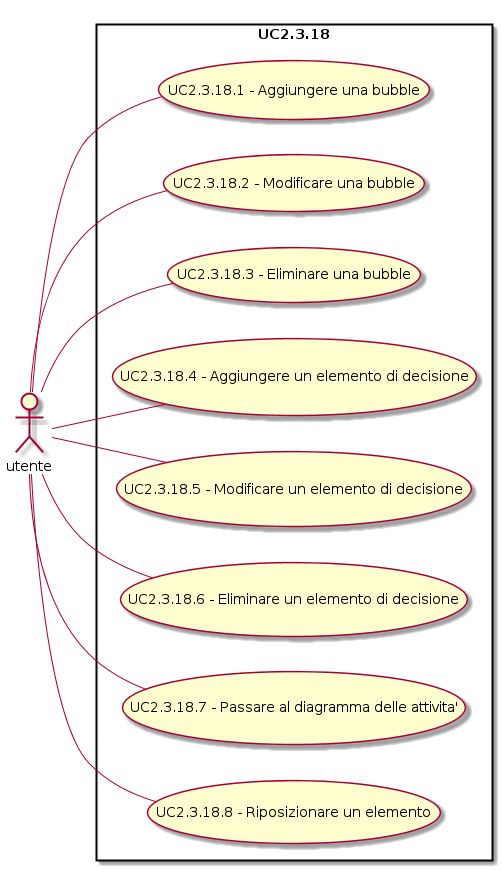
\includegraphics[scale=0.45]{./Figures/UC2-3-18.png}
						\caption{Diagramma UC2.3.18}\label{}
					\end{figure}
					\begin{itemize}
						\item \textbf{Attori}: Utente
						\item \textbf{Descrizione}: L'utente vuole editare un bubble flowchart;
						\item \textbf{Precondizione}: Nella schermata dell'editor del bubble flowchart il sistema è pronto a ricevere un comando dall'utente;
						\item \textbf{Flusso principale degli eventi}: \begin{itemize}
							\item L'utente può aggiungere una bubble (UC2.3.18.1);
							\item L'utente può modificare una bubble (UC2.3.18.2);
							\item L'utente può eliminare una bubble (UC2.3.18.3);
							\item L'utente può aggiungere un elemento di decisione (UC2.3.18.4);
							\item L'utente può modificare un elemento di decisione (UC2.3.18.5);
							\item L'utente può eliminare un elemento di decisione (UC2.3.18.6);
							\item L'utente può passare dal bubble flowchart al diagramma delle attività (UC2.3.18.7);
							\item L'utente può riposizionare un elemento (UC2.3.18.8);
						\end{itemize}
						\item \textbf{Postcondizione}: L'utente ha editato il bubble flowchart come voluto e il sistema è pronto a ricevere un nuovo comando.
					\end{itemize}
					\subsection{Caso d'uso UC2.3.18.1: Aggiungere una bubble}
					\begin{itemize}
						\item \textbf{Attori}: Utente
						\item \textbf{Descrizione}: L'utente vuole aggiungere una bubble di un tipo desiderato al bubble flowchart;
						\item \textbf{Precondizione}: Nella schermata dell'editor del bubble flowchart il sistema è pronto per l'aggiunta di una bubble;
						\item \textbf{Flusso principale degli eventi}: L'utente aggiunge una bubble di un tipo desiderato al bubble flowchart;
						\item \textbf{Postcondizione}: Nella schermata dell'editor del bubble flowchart è visualizzato il diagramma a cui è stata aggiunta una bubble vuota del tipo voluto.
					\end{itemize}
					\subsection{Caso d'uso UC2.3.18.2: Modificare una bubble}
					\begin{itemize}
						\item \textbf{Attori}: Utente
						\item \textbf{Descrizione}: L'utente vuole modificare i parametri di una bubble. Questi saranno specifici per ciascuna bubble, i relativi casi d'uso saranno quindi approfonditi nelle successive fasi di progettazione;
						\item \textbf{Precondizione}: Nella schermata dell'editor del bubble flowchart è stata selezionata una bubble;
						\item \textbf{Flusso principale degli eventi}: L'utente modifica i parametri di una bubble;
						\item \textbf{Scenari alternativi}: Viene annullata la modifica, il sistema	rimane nello stato precedente al tentativo di modifica;
						\item \textbf{Postcondizione}: Nella schermata dell'editor del bubble flowchart è visualizzato il diagramma in cui sono stati opportunamente modificati i parametri della bubble.
					\end{itemize}
					\subsection{Caso d'uso UC2.3.18.3: Eliminare una bubble}
					\begin{itemize}
						\item \textbf{Attori}: Utente
						\item \textbf{Descrizione}: L'utente vuole eliminare una bubble;
						\item \textbf{Precondizione}: Nella schermata dell'editor del bubble flowchart è stata selezionata una bubble;
						\item \textbf{Flusso principale degli eventi}: L'utente elimina una bubble;
						\item \textbf{Postcondizione}: Nella schermata dell'editor del bubble flowchart è visualizzato il diagramma in cui è stata eliminata la bubble.
					\end{itemize}
					\subsection{Caso d'uso UC2.3.18.4: Aggiungere un elemento di decisione}
					\begin{itemize}
						\item \textbf{Attori}: Utente
						\item \textbf{Descrizione}: L'utente vuole aggiungere un elemento di decisione al bubble flowchart;
						\item \textbf{Precondizione}: Nella schermata dell'editor del bubble flowchart il sistema è pronto per l'aggiunta di un elemento di decisione;
						\item \textbf{Flusso principale degli eventi}: L'utente aggiunge un elemento di decisione al bubble flowchart;
						\item \textbf{Postcondizione}: Nella schermata dell'editor del bubble flowchart è visualizzato il diagramma a cui è stato aggiunto un elemento di decisione vuoto.
					\end{itemize}
					\subsection{Caso d'uso UC2.3.18.5: Modificare un elemento di decisione}
					\begin{itemize}
						\item \textbf{Attori}: Utente
						\item \textbf{Descrizione}: L'utente vuole modificare i parametri di un elemento di decisione;
						\item \textbf{Precondizione}: Nella schermata dell'editor del bubble flowchart è stato selezionato un elemento di decisione;
						\item \textbf{Flusso principale degli eventi}: L'utente modifica i parametri di un elemento di decisione;
						\item \textbf{Postcondizione}: Nella schermata dell'editor del bubble flowchart è visualizzato il diagramma in cui sono stati opportunamente modificati i parametri dell'elemento di decisione.
					\end{itemize}
					\subsection{Caso d'uso UC2.3.18.6: Eliminare un elemento di decisione}
					\begin{itemize}
						\item \textbf{Attori}: Utente
						\item \textbf{Descrizione}: L'utente vuole eliminare un elemento di decisione;
						\item \textbf{Precondizione}: Nella schermata dell'editor del bubble flowchart è stato selezionato un elemento di decisione;
						\item \textbf{Flusso principale degli eventi}: L'utente elimina un elemento di decisione;
						\item \textbf{Postcondizione}: Nella schermata dell'editor del bubble flowchart è visualizzato il diagramma in cui è stato eliminato l'elemento di decisione.
					\end{itemize}
					\subsection{Caso d'uso UC2.3.18.7: Passare dal bubble flowchart al diagramma delle attività}
					\begin{itemize}
						\item \textbf{Attori}: Utente
						\item \textbf{Descrizione}: L'utente vuole tornare alla schermata dell'editor del diagramma delle attività;
						\item \textbf{Precondizione}: Il sistema visualizza l'editor del bubble flowchart;
						\item \textbf{Flusso principale degli eventi}: L'utente torna alla schermata dell'editor del diagramma delle attività;
						\item \textbf{Postcondizione}: Il sistema visualizza l'editor del diagramma delle attività.
					\end{itemize}
					\subsection{Caso d'uso UC2.3.18.8: Riposizionare un elemento}
					\begin{itemize}
						\item \textbf{Attori}: Utente
						\item \textbf{Descrizione}: L'utente vuole cambiare la posizione di un elemento all'interno del diagramma;
						\item \textbf{Precondizione}: L'utente si trova nella schermata dell'editor del bubble flowchart e il sistema è pronto a ricevere un comando dall'utente;
						\item \textbf{Flusso principale degli eventi}: L'utente riposiziona l'elemento;
						\item \textbf{Postcondizione}: Il sistema visualizza il diagramma con l'elemento riposizionato correttamente;
					\end{itemize}
					\subsection{Caso d'uso UC3: Gestire gli errori dell'utente}
					\begin{figure} [H]
						\centering
						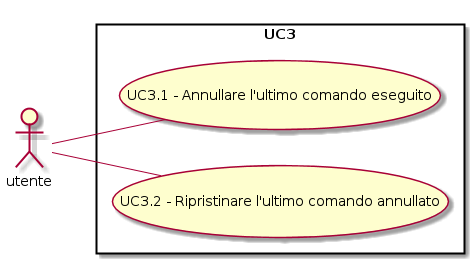
\includegraphics[scale=0.45]{./Figures/UC3.png}
						\caption{Diagramma UC3}\label{}
					\end{figure}
					\begin{itemize}
						\item \textbf{Attori}: Utente
						\item \textbf{Descrizione}: L'utente vuole gestire un errore che ha commesso utilizzando il programma;
						\item \textbf{Precondizione}: L'utente ha commesso un errore;
						\item \textbf{Flusso principale degli eventi}: \begin{itemize}
							\item L'utente può annullare l'ultimo comando eseguito (UC3.1);
							\item L'utente può ripristinare l'ultimo comando annullato (UC3.2);
						\end{itemize}
						\item \textbf{Postcondizione}: L'errore è stato gestito correttamente.
					\end{itemize}
					\subsection{Caso d'uso UC3.1: Annullare l'ultimo comando eseguito}
					\begin{itemize}
						\item \textbf{Attori}: Utente
						\item \textbf{Descrizione}: L'utente vuole annullare l'effetto dell'ultimo comando eseguito nell'editor del diagramma correntemente in uso;
						\item \textbf{Precondizione}: L'utente sta utilizzando l'editor di un diagramma tra quelli disponibili, ha eseguito almeno un comando e il sistema lo ha memorizzato;
						\item \textbf{Flusso principale degli eventi}: L'utente annulla l'effetto dell'ultimo comando eseguito nell'editor del diagramma correntemente in uso;
						\item \textbf{Postcondizione}: Il sistema ha ripristinato lo stato in cui si trovava il diagramma, correntemente in uso, prima che venisse eseguito il comando che è stato annullato; Il sistema ha memorizzato tale comando.
					\end{itemize}
					\subsection{Caso d'uso UC3.2: Ripristinare l'ultimo comando annullato}
					\begin{itemize}
						\item \textbf{Attori}: Utente
						\item \textbf{Descrizione}: L'utente vuole ripristinare l'effetto dell'ultimo comando precedentemente annullato nell'editor del diagramma correntemente in uso;
						\item \textbf{Precondizione}: Il programma è in esecuzione con un progetto aperto ed è appena stato annullato un comando;
						\item \textbf{Flusso principale degli eventi}: L'utente ripristina l'effetto dell'ultimo comando precedentemente annullato nell'editor del diagramma correntemente in uso;
						\item \textbf{Postcondizione}: Il programma è tornato nello stato precedente all'annullamento.
					\end{itemize}
					\subsection{Caso d'uso UC4: Gestire il codice generato}
					\begin{figure} [H]
						\centering
						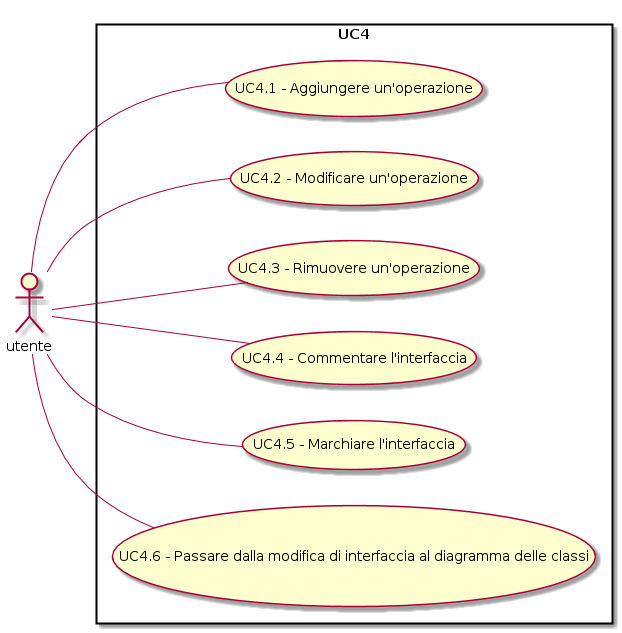
\includegraphics[scale=0.45]{./Figures/UC4.png}
						\caption{Diagramma UC4}\label{}
					\end{figure}
					\begin{itemize}
						\item \textbf{Attori}: Utente
						\item \textbf{Descrizione}: L'utente vuole gestire il codice generato dal programma;
						\item \textbf{Precondizione}: Il sistema è pronto a gestire il codice ed è in attesa di un comando da parte dell'utente;
						\item \textbf{Flusso principale degli eventi}: \begin{itemize}
							\item L'utente può leggere il codice prodotto (UC4.1);
							\item L'utente può esportare il codice prodotto (UC4.2);
						\end{itemize}
						\item \textbf{Postcondizione}: L'utente ha gestito correttamente il codice;
					\end{itemize}
					\subsection{Caso d'uso UC4.1: Leggere il codice prodotto}
					\begin{itemize}
						\item \textbf{Attori}: Utente
						\item \textbf{Descrizione}: L'utente vuole leggere il codice;
						\item \textbf{Precondizione}: Il sistema è pronto a mostrare il codice prodotto e in attesa di un comando da parte dell'utente;
						\item \textbf{Flusso principale degli eventi}: L'utente legge il codice;
						\item \textbf{Postcondizione}: Nella schermata del visualizzatore del codice è mostrato il codice prodotto.
					\end{itemize}
					\subsection{Caso d'uso UC4.2: Esportare il codice prodotto}
					\begin{itemize}
						\item \textbf{Attori}: Utente
						\item \textbf{Descrizione}: L'utente vuole esportare il codice generato nei file sorgente appropriati per il linguaggio corrispondente;
						\item \textbf{Precondizione}: Nelle schermate degli editor messi a disposizione del programma sono stati disegnati i diagrammi che rappresentano il codice desiderato;
						\item \textbf{Flusso principale degli eventi}: L'utente esporta il codice generato nei file sorgente appropriati per il linguaggio corrispondente;
						\item \textbf{Postcondizione}: In una cartella a scelta dell'utente il programma ha generato tutti i file sorgenti voluti, organizzati secondo quanto specificato dall'utente tramite i diagrammi. Questi file contengono codice corretto e compilabile. Qualora il programma non avesse potuto tradurre efficacemente una parte del diagramma dell'utente, il programma ha comunicato un avvertimento all'utente e commentato opportunamente il codice nel sorgente;
					\end{itemize}
\end{document}